% Options for packages loaded elsewhere
\PassOptionsToPackage{unicode}{hyperref}
\PassOptionsToPackage{hyphens}{url}
\documentclass[
  english,
  9pt,
]{extarticle}
\usepackage{xcolor}
\usepackage[margin=2cm]{geometry}
\usepackage{amsmath,amssymb}
\setcounter{secnumdepth}{5}
\usepackage{iftex}
\ifPDFTeX
  \usepackage[T1]{fontenc}
  \usepackage[utf8]{inputenc}
  \usepackage{textcomp} % provide euro and other symbols
\else % if luatex or xetex
  \usepackage{unicode-math} % this also loads fontspec
  \defaultfontfeatures{Scale=MatchLowercase}
  \defaultfontfeatures[\rmfamily]{Ligatures=TeX,Scale=1}
\fi
% \usepackage{lmodern}
\ifPDFTeX\else
  % xetex/luatex font selection
\fi
% Use upquote if available, for straight quotes in verbatim environments
\IfFileExists{upquote.sty}{\usepackage{upquote}}{}
\IfFileExists{microtype.sty}{% use microtype if available
  \usepackage[]{microtype}
  \UseMicrotypeSet[protrusion]{basicmath} % disable protrusion for tt fonts
}{}
\makeatletter
\@ifundefined{KOMAClassName}{% if non-KOMA class
  \IfFileExists{parskip.sty}{%
    \usepackage{parskip}
  }{% else
    \setlength{\parindent}{0pt}
    \setlength{\parskip}{6pt plus 2pt minus 1pt}}
}{% if KOMA class
  \KOMAoptions{parskip=half}}
\makeatother
\usepackage{color}
\usepackage{fancyvrb}
\newcommand{\VerbBar}{|}
\newcommand{\VERB}{\Verb[commandchars=\\\{\}]}
\DefineVerbatimEnvironment{Highlighting}{Verbatim}{commandchars=\\\{\}}
% Add ',fontsize=\small' for more characters per line
\newenvironment{Shaded}{}{}
\newcommand{\AlertTok}[1]{\textcolor[rgb]{1.00,0.00,0.00}{\textbf{#1}}}
\newcommand{\AnnotationTok}[1]{\textcolor[rgb]{0.38,0.63,0.69}{\textbf{\textit{#1}}}}
\newcommand{\AttributeTok}[1]{\textcolor[rgb]{0.49,0.56,0.16}{#1}}
\newcommand{\BaseNTok}[1]{\textcolor[rgb]{0.25,0.63,0.44}{#1}}
\newcommand{\BuiltInTok}[1]{\textcolor[rgb]{0.00,0.50,0.00}{#1}}
\newcommand{\CharTok}[1]{\textcolor[rgb]{0.25,0.44,0.63}{#1}}
\newcommand{\CommentTok}[1]{\textcolor[rgb]{0.38,0.63,0.69}{\textit{#1}}}
\newcommand{\CommentVarTok}[1]{\textcolor[rgb]{0.38,0.63,0.69}{\textbf{\textit{#1}}}}
\newcommand{\ConstantTok}[1]{\textcolor[rgb]{0.53,0.00,0.00}{#1}}
\newcommand{\ControlFlowTok}[1]{\textcolor[rgb]{0.00,0.44,0.13}{\textbf{#1}}}
\newcommand{\DataTypeTok}[1]{\textcolor[rgb]{0.56,0.13,0.00}{#1}}
\newcommand{\DecValTok}[1]{\textcolor[rgb]{0.25,0.63,0.44}{#1}}
\newcommand{\DocumentationTok}[1]{\textcolor[rgb]{0.73,0.13,0.13}{\textit{#1}}}
\newcommand{\ErrorTok}[1]{\textcolor[rgb]{1.00,0.00,0.00}{\textbf{#1}}}
\newcommand{\ExtensionTok}[1]{#1}
\newcommand{\FloatTok}[1]{\textcolor[rgb]{0.25,0.63,0.44}{#1}}
\newcommand{\FunctionTok}[1]{\textcolor[rgb]{0.02,0.16,0.49}{#1}}
\newcommand{\ImportTok}[1]{\textcolor[rgb]{0.00,0.50,0.00}{\textbf{#1}}}
\newcommand{\InformationTok}[1]{\textcolor[rgb]{0.38,0.63,0.69}{\textbf{\textit{#1}}}}
\newcommand{\KeywordTok}[1]{\textcolor[rgb]{0.00,0.44,0.13}{\textbf{#1}}}
\newcommand{\NormalTok}[1]{#1}
\newcommand{\OperatorTok}[1]{\textcolor[rgb]{0.40,0.40,0.40}{#1}}
\newcommand{\OtherTok}[1]{\textcolor[rgb]{0.00,0.44,0.13}{#1}}
\newcommand{\PreprocessorTok}[1]{\textcolor[rgb]{0.74,0.48,0.00}{#1}}
\newcommand{\RegionMarkerTok}[1]{#1}
\newcommand{\SpecialCharTok}[1]{\textcolor[rgb]{0.25,0.44,0.63}{#1}}
\newcommand{\SpecialStringTok}[1]{\textcolor[rgb]{0.73,0.40,0.53}{#1}}
\newcommand{\StringTok}[1]{\textcolor[rgb]{0.25,0.44,0.63}{#1}}
\newcommand{\VariableTok}[1]{\textcolor[rgb]{0.10,0.09,0.49}{#1}}
\newcommand{\VerbatimStringTok}[1]{\textcolor[rgb]{0.25,0.44,0.63}{#1}}
\newcommand{\WarningTok}[1]{\textcolor[rgb]{0.38,0.63,0.69}{\textbf{\textit{#1}}}}
\usepackage{longtable,booktabs,array}
\usepackage{caption}
\captionsetup[table]{skip=6pt}
\newcounter{none} % for unnumbered tables
\usepackage{calc} % for calculating minipage widths
% Correct order of tables after \paragraph or \subparagraph
\usepackage{etoolbox}
\makeatletter
\patchcmd\longtable{\par}{\if@noskipsec\mbox{}\fi\par}{}{}
\makeatother
% Allow footnotes in longtable head/foot
\IfFileExists{footnotehyper.sty}{\usepackage{footnotehyper}}{\usepackage{footnote}}
\makesavenoteenv{longtable}
\usepackage{graphicx}
\makeatletter
\newsavebox\pandoc@box
\newcommand*\pandocbounded[1]{% scales image to fit in text height/width
  \sbox\pandoc@box{#1}%
  \Gscale@div\@tempa{\textheight}{\dimexpr\ht\pandoc@box+\dp\pandoc@box\relax}%
  \Gscale@div\@tempb{\linewidth}{\wd\pandoc@box}%
  \ifdim\@tempb\p@<\@tempa\p@\let\@tempa\@tempb\fi% select the smaller of both
  \ifdim\@tempa\p@<\p@\scalebox{\@tempa}{\usebox\pandoc@box}%
  \else\usebox{\pandoc@box}%
  \fi%
}
% Set default figure placement to htbp
\def\fps@figure{htbp}
\makeatother
\ifLuaTeX
\usepackage[bidi=basic,shorthands=off]{babel}
\else
\usepackage[bidi=default,shorthands=off]{babel}
\fi
\ifLuaTeX
  \usepackage{selnolig} % disable illegal ligatures
\fi
\setlength{\emergencystretch}{3em} % prevent overfull lines
\providecommand{\tightlist}{%
  \setlength{\itemsep}{0pt}\setlength{\parskip}{0pt}}
\usepackage[]{natbib}
\bibliographystyle{plainnat}
\makeatletter
\@ifpackageloaded{subcaption}{}{\usepackage{subcaption}}
\@ifpackageloaded{caption}{}{\usepackage{caption}}
\captionsetup[subfigure]{margin=0.5em}
\AtBeginDocument{%
\renewcommand*\figurename{Figure}
\renewcommand*\tablename{Table}
}
\AtBeginDocument{%
\renewcommand*\listfigurename{List of Figures}
\renewcommand*\listtablename{List of Tables}
}
\newcounter{pandoccrossref@subfigures@footnote@counter}
\newenvironment{pandoccrossrefsubfigures}{%
\setcounter{pandoccrossref@subfigures@footnote@counter}{0}
\begin{figure}\centering%
\gdef\global@pandoccrossref@subfigures@footnotes{}%
\DeclareRobustCommand{\footnote}[1]{\footnotemark%
\stepcounter{pandoccrossref@subfigures@footnote@counter}%
\ifx\global@pandoccrossref@subfigures@footnotes\empty%
\gdef\global@pandoccrossref@subfigures@footnotes{{##1}}%
\else%
\g@addto@macro\global@pandoccrossref@subfigures@footnotes{, {##1}}%
\fi}}%
{\end{figure}%
\addtocounter{footnote}{-\value{pandoccrossref@subfigures@footnote@counter}}
\@for\f:=\global@pandoccrossref@subfigures@footnotes\do{\stepcounter{footnote}\footnotetext{\f}}%
\gdef\global@pandoccrossref@subfigures@footnotes{}}
\@ifpackageloaded{float}{}{\usepackage{float}}
\floatstyle{ruled}
\@ifundefined{c@chapter}{\newfloat{codelisting}{h}{lop}}{\newfloat{codelisting}{h}{lop}[chapter]}
\floatname{codelisting}{Listing}
\newcommand*\listoflistings{\listof{codelisting}{List of Listings}}
\makeatother
\usepackage{bookmark}
\IfFileExists{xurl.sty}{\usepackage{xurl}}{} % add URL line breaks if available
\urlstyle{same}
% fallback for those not using the hyperref driver hyperxmp:
\makeatletter
\@ifundefined{xmpquote}{\newcommand{\xmpquote}[1]{#1}}{}
\makeatother
\hypersetup{
  pdftitle={GeneralizedNotationNotation: A Text Language for Active Inference Models},
  pdfauthor={Daniel Ari Friedman},
  pdflang={en},
  colorlinks=true,linkcolor=red,urlcolor=red,citecolor=red,anchorcolor=red,filecolor=red,
  pdfcreator={LaTeX via pandoc}}

\title{GeneralizedNotationNotation: A Text Language for Active Inference
Models}
\author{Daniel Ari Friedman}
\date{}

\IfFileExists{seqsplit.sty}{\usepackage{seqsplit}}{\newcommand{\seqsplit}[1]{#1}}
\protected\def\breakseq#1{\seqsplit{#1}}
\protected\def\breaktt#1{\begingroup\ttfamily\seqsplit{#1}\endgroup}
\title{GeneralizedNotationNotation: A Text Language for Active Inference Models}
\author{Daniel Ari Friedman}
\date{2026-09-06}

\usepackage{amsmath}
\usepackage{amssymb}
\usepackage{geometry}
\usepackage{graphicx}
\usepackage{booktabs}
\usepackage{longtable}
\usepackage{array}
\usepackage{hyperref}
\usepackage{natbib}

% Contents listing: article.cls prefixes every \l@section entry with
% \addvspace{1.0em}, which across ten sections costs about ten lines and pushed
% the ~40-entry listing one line past page 2 — leaving a third sheet carrying a
% single "10 References" line. Tighten that inter-section gap for the duration
% of \tableofcontents only, inside a group, so body spacing is untouched and no
% entry is dropped (reducing \tocdepth would have hidden 29 real subsections).
\makeatletter
\let\GNNoriginaltableofcontents\tableofcontents
\renewcommand{\tableofcontents}{%
  \begingroup
  \setlength{\parskip}{0pt}%
  \renewcommand{\addvspace}[1]{\vskip 2\p@}%
  \GNNoriginaltableofcontents
  \endgroup}
\makeatother
% Document metadata. config.yaml declares a subtitle and a keyword list, and
% the producer emits both as tokens, but the template's \hypersetup writes only
% pdftitle/pdfauthor/pdflang -- so `pdfinfo` reported no Subject and no
% Keywords. This block runs after the template's, so it wins.
%
% The two values below are WRITTEN by scripts/z_generate_manuscript_variables.py
% (sync_preamble_metadata), never typed. A double-brace token cannot be used here:
% preamble.md is substituted into output/manuscript/ like any other section, but
% the template's _manuscript_source.py then copies the raw file back over that
% copy, so an unresolved token would reach hyperref and land in the PDF's
% metadata verbatim.
\hypersetup{
  pdfsubject={A text language and modular processing pipeline for Active Inference generative models},
  pdfkeywords={GNN, active inference, generative models, model notation, pipeline automation}}

% Bounded identifier splitting. The template defines
%   \protected\def\breaktt#1{\begingroup\ttfamily\seqsplit{#1}\endgroup}
% and \seqsplit permits a break after EVERY character with no continuation cue.
% In the 2026-09-05 PDF that rendered `model_family_manifest.json` as
% `model_family_manifest.js` + `on` and `src/manuscript_variables.py` as
% `(src/manusc` + `ript_variables.py` — the first is itself a valid filename, so
% a reader cannot tell a line break from a name. Keep seqsplit's guarantee that
% no code token overflows the measure, but forbid breaks inside the last
% \GNNttTail characters (an extension is never orphaned) and inside the first
% \GNNttHead (a one- or two-letter stub is never left behind).
\makeatletter
\newcount\GNN@ttlen
\newcount\GNN@ttpos
\newcount\GNN@ttleft
\def\GNNttHead{2}
\def\GNNttTail{5}
\def\GNN@ttstop{}
\long\def\GNN@ttcount#1{%
  \ifx#1\GNN@ttstop \let\GNN@ttnext\relax
  \else \advance\GNN@ttlen\@ne \let\GNN@ttnext\GNN@ttcount \fi
  \GNN@ttnext}
\long\def\GNN@ttemit#1{%
  \ifx#1\GNN@ttstop \let\GNN@ttnext\relax
  \else
    #1%
    \advance\GNN@ttpos\@ne
    \GNN@ttleft\GNN@ttlen \advance\GNN@ttleft-\GNN@ttpos
    \ifnum\GNN@ttpos>\GNNttHead
      \ifnum\GNN@ttleft>\GNNttTail \discretionary{}{}{}\fi
    \fi
    \let\GNN@ttnext\GNN@ttemit
  \fi
  \GNN@ttnext}
\protected\def\breaktt#1{%
  \begingroup
  \ttfamily
  \GNN@ttlen\z@ \GNN@ttcount#1\GNN@ttstop
  \GNN@ttpos\z@ \GNN@ttemit#1\GNN@ttstop
  \endgroup}
\makeatother
\usepackage{listings}
\lstset{basicstyle=\ttfamily\small,breaklines=true,columns=fullflexible}
\newtheorem{theorem}{Theorem}[section]
\newtheorem{remark}[theorem]{Remark}
\newtheorem{example}[theorem]{Example}

\begin{document}
\begin{titlepage}
\centering
\vspace*{0.55cm}
{\Huge\sffamily\bfseries GeneralizedNotationNotation: A Text Language for Active Inference Models\par}
\vspace{0.4em}
{\Large\sffamily A text language and modular processing pipeline for Active Inference generative models\par}
\vspace{0.75em}
{\large\sffamily\bfseries Daniel Ari Friedman\par}
{\small\sffamily Active Inference Institute\par}
{\small\sffamily\texttt{daniel@activeinference.institute}\par}
{\small\sffamily\href{https://orcid.org/0000-0001-6232-9096}{ORCID: 0000-0001-6232-9096}\par}
\vspace{0.08em}
{\small\sffamily DOI: \href{https://doi.org/10.5281/zenodo.7803327}{10.5281/zenodo.7803327}\par}
\vspace{0.35em}
\makeatletter
{\@date\par}
\makeatother
\vfill

\includegraphics[width=0.98\textwidth,height=0.6\textheight,keepaspectratio,alt={Graphical abstract: one plain-text GNN specification flowing through parse, validate, render, execute, and analyze cards into cross-repository interchange checks against the pinned GEO-INFER and fep-lean pairs.}]{\detokenize{../figures/gnn_graphical_abstract.png}}
\vfill
\end{titlepage}
\thispagestyle{empty}
\tableofcontents
\newpage

\section{Abstract}\label{sec:abstract}

\begin{figure}
\centering
\includegraphics[width=1\linewidth,height=0.5\textheight,keepaspectratio,alt={The GeneralizedNotationNotation (GNN) pipeline at a glance, generated from the producer's token map at commit 13bd0637c. A plain-text specification --- the StateSpaceBlock declaring the model's tensors, A, B, C, D, and E for the discrete categorical kind of eq.~ through eq.~ and its own matrix vocabulary for the other model kinds --- is parsed (Step 3), type-checked and validated (Steps 5--6), rendered as backend-specific code (Step 11), executed (Step 12), and analyzed (Step 16), before artifacts flow into the cross-repository interchange checks against the pinned GEO-INFER and fep\_lean pairs. Read the cards left to right: each header names the stage, each pill names the pipeline step (or the source role), and the body states what the stage produces. The validation stage includes the B-tensor orientation check --- every discrete B literal is read as column-stochastic B{[}s\textquotesingle, s, a{]}, and -\/-transpose-b maps row-stochastic textbook literals onto that canonical order --- and the execution stage includes the bnlearn lane, which generates runnable Python from the same parsed model and skips with a recorded status when its runtime is absent. The footer states the scale the panel summarizes: 25 pipeline steps, 9 model families, 9 registered render backends with all 9 executing at Step 12, and 142 Model Context Protocol tools.}]{../figures/gnn_graphical_abstract.png}
\caption{The GeneralizedNotationNotation (GNN) pipeline at a glance,
generated from the producer's token map at commit 13bd0637c. A
plain-text specification --- the \protect\texttt{StateSpaceBlock}
declaring the model's tensors, \protect\texttt{A}, \protect\texttt{B},
\protect\texttt{C}, \protect\texttt{D}, and \protect\texttt{E} for the
discrete categorical kind of eq.~\ref{eq:generative_model} through
eq.~\ref{eq:policy} and its own matrix vocabulary for the other model
kinds --- is parsed (Step 3), type-checked and validated (Steps 5--6),
rendered as backend-specific code (Step 11), executed (Step 12), and
analyzed (Step 16), before artifacts flow into the cross-repository
interchange checks against the pinned GEO-INFER and fep\_lean pairs.
Read the cards left to right: each header names the stage, each pill
names the pipeline step (or the source role), and the body states what
the stage produces. The validation stage includes the B-tensor
orientation check --- every discrete \protect\texttt{B} literal is read
as column-stochastic
\protect\texttt{B{[}s\textquotesingle{},\ s,\ a{]}}, and
\protect\texttt{-\/-transpose-b} maps row-stochastic textbook literals
onto that canonical order --- and the execution stage includes the
bnlearn lane, which generates runnable Python from the same parsed model
and skips with a recorded status when its runtime is absent. The footer
states the scale the panel summarizes: 25 pipeline steps, 9 model
families, 9 registered render backends with all 9 executing at Step 12,
and 142 Model Context Protocol tools.}\label{fig:graphical_abstract}
\end{figure}

Active Inference offers a unifying account of perception, learning, and
action under the free energy principle \citep{friston2010}, yet the
generative models at its core are still communicated ad hoc: scattered
across prose descriptions, bespoke notebooks, and framework-specific
code that rarely agree. This fragmentation makes published models hard
to reproduce, compare, or port between tools, and it raises the barrier
for newcomers learning the formalism \citep{parr2022}.
GeneralizedNotationNotation (GNN) addresses this gap with a
standardized, human- and machine-readable text language for specifying
Active Inference generative models, paired with a 25-step processing
pipeline that transforms a single specification into validation,
visualization, simulation, and analysis artifacts \citep{gnn2023}. A GNN
file denotes a generative model, and the language lets that model take
the several shapes the field actually uses: the notation blocks a file
declares --- categorical
\texttt{A}/\texttt{B}/\texttt{C}/\texttt{D}{[}/\texttt{E}{]} tensors,
linear-Gaussian system matrices
\texttt{F}/\texttt{H}/\texttt{Q}/\texttt{R} with a Gaussian prior,
per-agent and per-level compositions --- fix its model kind, which the
pipeline classifies structurally and carries through rendering and
execution, recording explicitly which registered backends can render and
run a model of each kind and which report it unsupported. GNN's ``Triple
Play'' treats each model as three coordinated views --- a textual
specification, graphical visualizations, and executable cognitive models
--- so that one source yields consistent outputs across modalities. The
framework spans 30 exemplar specifications (27 discrete-state and 3
continuous linear-Gaussian) across 9 model families and 9 registered
rendering backends, with explicit gates for cross-format semantic
fidelity and cross-framework reliability. GNN 3.0.0 layered
safe-by-design long-running orchestration on top of this language and
pipeline --- durable observation streams, resumable run sessions, and
auditable container plans that generate, validate, and replay data only,
with no live infrastructure mutation. We describe the language, the
model kinds it denotes, the pipeline architecture, and the validation
that confirms specifications round-trip faithfully across formats and
execute across multiple simulation backends --- with coverage gaps
recorded as explicit profiled-unsupported statuses rather than silently
omitted --- establishing GNN as reproducible, interoperable
infrastructure for communicating Active Inference models.

\newpage

\section{Introduction}\label{sec:introduction}

\subsection{Motivation}\label{motivation}

Active Inference has matured into a broad research program spanning the
free energy principle \citep{friston2010}, discrete state-space
formulations of perception and action \citep{dacosta2020}, and a growing
body of pedagogy and reference implementations
\citep{parr2022, smith2022}. Recent graphical-specification and
message-passing work makes the same practical pressure visible:
active-inference agents need representations that can be inspected as
model structure and then carried into executable inference updates
without being reauthored by hand
\citep{koudahl2023syntheticAgents1, vandelaaar2023syntheticAgents2, bagaev2021reactiveMessagePassing}.
As the field has grown, so has a quieter problem: the models themselves
are difficult to share, reproduce, and compare. A generative model that
lives only as a tangle of matrix definitions inside one author's script,
a diagram in a slide deck, and a paragraph of prose in a paper has no
single authoritative form. The same model is described three times, in
three incompatible media, with no guarantee that they agree. When a
reader wants to re-run that model in a different toolkit, they must
reverse-engineer it from whichever fragment they happen to have.

This is a reproducibility and interoperability crisis specific to the
structure of Active Inference work. The discipline depends on precisely
specified state spaces, observation and transition tensors, prior
preferences, and policy structures; small notational ambiguities
propagate into materially different behaviour. The heterogeneity of the
models themselves compounds the problem: the field works in several
model kinds at once --- discrete categorical POMDPs over finite state
spaces, continuous linear-Gaussian state-space models, multi-agent
systems whose agents each carry their own generative vocabulary,
hierarchical compositions layered over timescales --- and each kind
attracts its own notation, its own notebooks, and its own simulation
stack. Yet the community has lacked a notation that is simultaneously
human-readable, machine-parseable, and faithful to the underlying
mathematics across those kinds. Generalized Notation Notation (GNN) was
introduced to fill exactly that gap \citep{gnn2023}: a standard,
text-based way to write down an Active Inference generative model once,
such that every downstream use derives from the same source of truth.

\subsection{The GNN Approach}\label{the-gnn-approach}

GNN treats the model specification as a first-class artifact. A model is
written in a plain-text language whose syntax captures the components an
Active Inference modeller actually reasons about --- state factors,
observation modalities, the matrices that link them, control structure,
and the temporal organization of the model --- and whose declared matrix
vocabulary fixes which kind of generative model the file denotes:
categorical \texttt{A}/\texttt{B}/\texttt{C}/\texttt{D}{[}/\texttt{E}{]}
tensors for a discrete state-space model, linear-Gaussian system
matrices for a continuous one, per-agent and per-level compositions for
structured variants. Because the specification is text, it lives
comfortably in version control, diffs cleanly across revisions, and can
be authored and reviewed by humans without specialized tooling.

The defining commitment of GNN is what the project calls the Triple
Play: a single text specification is the common origin for three
coordinated renderings of the same model. The text form is the
authoritative, editable description. From it, GNN produces graphical
visualizations that expose the model's factor and dependency structure
for inspection and communication. And from the same source it produces
executable cognitive models that can actually be run, so that the
diagram, the equations, and the running code are all generated from one
parsed document rather than three artifacts that merely claim to
describe the same model. The Triple Play turns a model from a
description scattered across media into one specification with multiple
faithful projections (see fig.~\ref{fig:triple_play}).

\subsection{Contributions}\label{contributions}

This work contributes a standard notation together with the
infrastructure that makes it usable in practice:

\begin{itemize}
\tightlist
\item
  \textbf{A parseable, human-readable notation} for Active Inference
  generative models, whose text form is authoritative and from which
  every other representation is derived.
\item
  \textbf{A model-kind taxonomy with per-kind rendering and execution
  semantics} --- discrete categorical, continuous linear-Gaussian,
  multi-agent, hierarchical, learning, and structural kinds, classified
  structurally from the declared notation and rendered or
  recorded-unsupported per backend --- so that what a specification can
  do on a given framework is a checkable property of the model's kind,
  not a trial-and-error discovery.
\item
  \textbf{A 25-step processing pipeline} (0--24), whose stages are
  implemented across 44 source packages, that carries a specification
  from parsing and validation through visualization, rendering, and
  execution.
\item
  \textbf{9 rendering backends} (PyMDP, RxInfer.jl, ActiveInference.jl,
  JAX, DisCoPy, PyTorch, NumPyro, Stan, bnlearn) that materialize a
  single GNN specification as backend-specific model code, of which 9
  (PyMDP, RxInfer.jl, ActiveInference.jl, JAX, DisCoPy, PyTorch,
  NumPyro, Stan, bnlearn) also execute at Step 12, realizing the
  executable arm of the Triple Play.
\item
  \textbf{142 Model Context Protocol tools} that expose the pipeline's
  capabilities to agentic and programmatic clients, so the notation and
  its tooling are directly accessible to automated workflows.
\item
  \textbf{9-family reliability gates} that exercise the pipeline against
  a curated set of model families (basics, discrete, continuous,
  hierarchical, multiagent, precision, structured, gridworld,
  scaling-study), turning interoperability claims into checks that must
  pass rather than assertions that are merely made.
\end{itemize}

\subsection{Reader Orientation}\label{reader-orientation}

The remainder of this manuscript is organized to move from language to
mechanism to evidence. sec.~\ref{sec:system_context} states the notation
and the model kinds it denotes --- the discrete categorical
factorization, its four matrices, and its two free-energy objectives as
explicit equations (eq.~\ref{eq:generative_model} through
eq.~\ref{eq:policy}), the continuous linear-Gaussian state-space kind
with its optional closed-loop control structure
(eq.~\ref{eq:lgssm_state} through eq.~\ref{eq:closed_loop}), and the
multi-agent, hierarchical, learning, and structural compositions --- and
it presents the model-kind table (tbl.~\ref{tbl:model_kinds}), the
pipeline structure (fig.~\ref{fig:pipeline}), the Triple Play
(fig.~\ref{fig:triple_play}), and the per-step responsibility table
(tbl.~\ref{tbl:pipeline_steps}). sec.~\ref{sec:methods} follows a
specification through the pipeline --- parsing, kind-scoped type
checking, rendering, execution, and reporting --- and presents the
backend registry (tbl.~\ref{tbl:backend_registry}), the per-kind
framework capability matrix (tbl.~\ref{tbl:framework_capability}), the
backend registry surface (fig.~\ref{fig:backend_matrix}), and the
long-running orchestration contracts (fig.~\ref{fig:orchestration}).
sec.~\ref{sec:artifacts_evidence} reports what the project has produced
and how each number is grounded, with the model-family registry
(tbl.~\ref{tbl:model_families}), the family-by-framework coverage
(fig.~\ref{fig:family_matrix}), and repository-scale metrics
(fig.~\ref{fig:repo_metrics}). fig.~\ref{fig:graphical_abstract}
condenses this same arc --- specification, validation, rendering,
execution, analysis, and interchange --- into the summary panel at the
head of the manuscript. Claims of independent re-execution are addressed
in sec.~\ref{sec:reproducibility}, the boundaries of the current system
in sec.~\ref{sec:limitations_next_steps}, the symbol and construct
tables in sec.~\ref{sec:symbols_glossary}, and full source details in
sec.~\ref{sec:references}. Read in this order, the manuscript moves from
why a standard notation is needed, through how GNN realizes it across
model kinds, to the evidence that the standard holds.

\newpage

\section{System Context}\label{sec:system_context}

Generalized Notation Notation (GNN) couples a small, declarative text
language for generative models in the Active Inference lineage to a
deterministic processing pipeline that turns each specification into
validation, visualization, simulation, and analysis artifacts
\citep{gnn2023}. The language gives a model one canonical written form;
the pipeline gives that form many executable and graphical realizations.
This section describes both halves of the architecture and the way they
meet, and it states the mathematical objects the language is obliged to
carry --- per model kind, because the language is not tied to a single
shape of generative model.

\subsection{The GNN Language}\label{the-gnn-language}

A GNN model is a plain-text document organized into named sections that
together pin down the generative model its author intends. The
\texttt{StateSpaceBlock} declares the variables of the model and their
dimensions --- hidden states, observations, control factors, policies,
or the system matrices of a continuous model --- establishing the shape
of every tensor that follows. The \texttt{Connections} section records
the directed and undirected dependencies among those variables, the
edges of the underlying factor graph that downstream tools read to lay
out diagrams and wire up inference. Which family of generative model a
file declares is decided by the notation the file carries, not by its
filename or its directory: the declared matrix vocabulary is what the
pipeline reads to classify the model, as sec.~\ref{sec:model_kinds}
specifies. The full construct vocabulary is catalogued in
tbl.~\ref{tbl:gnn_constructs}.

\subsection{Model Kinds}\label{sec:model_kinds}

Every GNN file denotes one generative model, and the language lets that
model take several distinct mathematical shapes. A file whose
\texttt{StateSpaceBlock} declares the categorical tensors \texttt{A},
\texttt{B}, \texttt{C}, \texttt{D} --- optionally \texttt{E} --- denotes
a discrete state-space generative model. A file that declares the system
matrices \texttt{F}, \texttt{H}, \texttt{Q}, \texttt{R} together with a
Gaussian prior over the initial state (\texttt{prior\_mean},
\texttt{prior\_cov}) denotes a continuous linear-Gaussian state-space
model. Per-agent and per-level declarations (\texttt{A\_agent1},
\texttt{A\_level1}, \ldots) compose the categorical vocabulary into
multi-agent and hierarchical structures. A file that declares boundary
structure only --- neither a categorical nor a continuous
parameterization --- is a structural wrapper: it names the model's
interfaces but carries no renderable form.

The pipeline classifies each parsed specification structurally, and it
does so from typed fields alone: the raw \texttt{\#\#\ GNNSection}
value, the declared matrix-key patterns, explicit agent counts, and
explicit \breaktt{\#\#\ ModelParameters} keys. The classifier
(\breaktt{detect\_model\_kind} in
\breaktt{src/gnn/render/pomdp\_contract.py}) resolves kinds in a fixed
precedence order --- multi-agent, then hierarchical, then continuous,
then learning, then factored, then structural, then the flat
single-factor case --- so the more specific structure wins when a file
exhibits several at once. Two properties of this classification matter
for everything downstream. First, it is structural, not textual: prose
in a model name or annotation never changes how a model renders, so a
passing mention of ``Dirichlet'' in free text cannot reroute a
specification into the parameter-learning kind. Second, it is computed
from the parsed specification, not asserted by the author: the same file
classifies the same way on every machine, which is what lets rendering
and execution behavior be stated per kind rather than per file. The
taxonomy, its notation blocks, exemplar folder, and rendering and
execution reach per kind are enumerated in tbl.~\ref{tbl:model_kinds}.

\begin{longtable}[]{@{}
  >{\raggedright\arraybackslash}p{(\linewidth - 8\tabcolsep) * \real{0.2000}}
  >{\raggedright\arraybackslash}p{(\linewidth - 8\tabcolsep) * \real{0.2000}}
  >{\raggedright\arraybackslash}p{(\linewidth - 8\tabcolsep) * \real{0.2000}}
  >{\raggedright\arraybackslash}p{(\linewidth - 8\tabcolsep) * \real{0.2000}}
  >{\raggedright\arraybackslash}p{(\linewidth - 8\tabcolsep) * \real{0.2000}}@{}}
\caption{The model kinds the pipeline represents and executes, one row
per kind. Notation blocks are the parameterization each kind declares;
exemplar folders are the committed corpus under
\protect\breaktt{input/gnn\_files/}. Renderer(s)/Executor(s) cells are
generated from the registry flags (see
tbl.~\ref{tbl:framework_capability}): the two parameterization rows
carry their own flag sets, and multi-agent inherits the discrete row's
coverage because its per-agent matrix keys canonicalize through the same
discrete A/B/C/D render path; \protect\texttt{recursive/} is reserved
for bounded \protect\texttt{-\/-autonomous} proposal-loop runs and holds
no committed models.}\label{tbl:model_kinds}\tabularnewline
\toprule\noalign{}
\begin{minipage}[b]{\linewidth}\raggedright
Model kind
\end{minipage} & \begin{minipage}[b]{\linewidth}\raggedright
Notation block
\end{minipage} & \begin{minipage}[b]{\linewidth}\raggedright
Exemplar folder
\end{minipage} & \begin{minipage}[b]{\linewidth}\raggedright
Renderer(s)
\end{minipage} & \begin{minipage}[b]{\linewidth}\raggedright
Executor(s)
\end{minipage} \\
\midrule\noalign{}
\endfirsthead
\toprule\noalign{}
\begin{minipage}[b]{\linewidth}\raggedright
Model kind
\end{minipage} & \begin{minipage}[b]{\linewidth}\raggedright
Notation block
\end{minipage} & \begin{minipage}[b]{\linewidth}\raggedright
Exemplar folder
\end{minipage} & \begin{minipage}[b]{\linewidth}\raggedright
Renderer(s)
\end{minipage} & \begin{minipage}[b]{\linewidth}\raggedright
Executor(s)
\end{minipage} \\
\midrule\noalign{}
\endhead
\bottomrule\noalign{}
\endlastfoot
Discrete categorical &
\texttt{A}/\texttt{B}/\texttt{C}/\texttt{D}{[}/\texttt{E}{]}
(column-stochastic \texttt{B} slices) &
\breaktt{input/gnn\_files/discrete/} & all 9 registry frameworks & all 9
registry frameworks \\
Continuous linear-Gaussian & \texttt{F}/\texttt{H}/\texttt{Q}/\texttt{R}
+ priors (optional closed-loop pair) &
\breaktt{input/gnn\_files/continuous/} & RxInfer.jl, JAX, PyTorch,
NumPyro, Stan & RxInfer.jl, JAX, PyTorch, NumPyro, Stan \\
Multi-agent & \texttt{nr\_agents} + per-agent matrix keys
(\texttt{A\_agent1}, \ldots) & \breaktt{input/gnn\_files/multiagent/} &
all 9 registry frameworks & all 9 registry frameworks \\
Recursive & --- & \breaktt{input/gnn\_files/recursive/} & --- & --- \\
\end{longtable}

\subsubsection{The Discrete Categorical
Kind}\label{the-discrete-categorical-kind}

A discrete specification denotes a partially observable Markov decision
process over a horizon \(T\), factorized as in
eq.~\ref{eq:generative_model} following the standard formulation
\citep{dacosta2020, smith2022}.

\begin{equation}\protect\phantomsection\label{eq:generative_model}{
P(o_{1:T},\, s_{1:T},\, \pi) \;=\; P(\pi)\; P(s_1) \prod_{t=1}^{T} P(o_t \mid s_t) \prod_{t=2}^{T} P(s_t \mid s_{t-1},\, \pi)
}\end{equation}

The four matrices named in the \texttt{StateSpaceBlock} are exactly the
factors of eq.~\ref{eq:generative_model}, and this correspondence is
what makes the notation translatable rather than merely descriptive. The
\texttt{A} matrix is the likelihood, a column-stochastic map from hidden
states to observation outcomes, given in eq.~\ref{eq:likelihood}.

\begin{equation}\protect\phantomsection\label{eq:likelihood}{
P(o_t = i \mid s_t = j) \;=\; A_{ij}, \qquad \sum_i A_{ij} = 1
}\end{equation}

The \texttt{B} matrix is the controlled transition dynamics: one
column-stochastic slice per action, as in eq.~\ref{eq:transition}. The
canonical reading of the tensor is column-stochastic,
\texttt{B{[}next\_state{]}{[}previous\_state{]}{[}action{]}}, matching
the convention of the discrete message-passing libraries the pipeline
targets \citep{heins2022}; validation records every declared tensor's
detected orientation and can transpose row-stochastic textbook literals
on request, as described in sec.~\ref{sec:methods}.

\begin{equation}\protect\phantomsection\label{eq:transition}{
P(s_{t+1} = i \mid s_t = j,\, u_t = k) \;=\; B^{(k)}_{ij}, \qquad \sum_i B^{(k)}_{ij} = 1
}\end{equation}

The \texttt{C} vector holds log-preferences over observations, which
enter inference as the biased outcome distribution of
eq.~\ref{eq:preference}; the \texttt{D} vector is the prior over initial
hidden states, eq.~\ref{eq:prior}.

\begin{equation}\protect\phantomsection\label{eq:preference}{
\tilde{P}(o_t = i) \;=\; \sigma(C)_i \;=\; \frac{\exp C_i}{\sum_j \exp C_j}
}\end{equation}

\begin{equation}\protect\phantomsection\label{eq:prior}{
P(s_1 = i) \;=\; D_i, \qquad \sum_i D_i = 1
}\end{equation}

Given those factors, perception is approximate Bayesian inference: a
variational posterior \(Q(s)\) is fitted by minimizing the variational
free energy of eq.~\ref{eq:vfe}, which decomposes into a complexity term
and an accuracy term \citep{friston2010}.

\begin{equation}\protect\phantomsection\label{eq:vfe}{
F[Q] \;=\; \underbrace{D_{\mathrm{KL}}\!\left[\,Q(s) \,\|\, P(s)\,\right]}_{\text{complexity}} \;-\; \underbrace{\mathbb{E}_{Q(s)}\!\left[\ln P(o \mid s)\right]}_{\text{accuracy}}
}\end{equation}

Action is expected-free-energy minimization: each policy \(\pi\) is
scored over future steps \(\tau\) by eq.~\ref{eq:efe}, whose two terms
are the information gain a policy is expected to yield and the extent to
which its predicted outcomes match \texttt{C} \citep{dacosta2020}.

\begin{equation}\protect\phantomsection\label{eq:efe}{
G(\pi) \;=\; -\underbrace{\mathbb{E}_{Q(o_\tau,\, s_\tau \mid \pi)}\!\left[\ln Q(s_\tau \mid o_\tau, \pi) - \ln Q(s_\tau \mid \pi)\right]}_{\text{epistemic value}} \;-\; \underbrace{\mathbb{E}_{Q(o_\tau \mid \pi)}\!\left[\ln \tilde{P}(o_\tau)\right]}_{\text{pragmatic value}}
}\end{equation}

The policy posterior then combines those scores with the habit prior
\texttt{E} declared in the specification, as in eq.~\ref{eq:policy}, and
the selected action \(u\) is sampled from it.

\begin{equation}\protect\phantomsection\label{eq:policy}{
Q(\pi) \;=\; \sigma\!\left(\ln E - G\right)
}\end{equation}

The discrete categorical kind is the language's original and most
densely exercised target: 27 of the 30 exemplar specifications in the
corpus are discrete-state. The discrete family folder holds the kind's
core set --- from minimal \texttt{markov\_chain.md} and
\texttt{hmm\_baseline.md} fixtures through epistemic planning
(\breaktt{tmaze\_epistemic.md}) and deep planning horizons
(\breaktt{deep\_planning\_horizon.md}) to the canonical full agent
(\breaktt{actinf\_pomdp\_agent.md}) --- and further categorical fixtures
populate the basics, precision, structured, gridworld, and scaling-study
corpora. The kind composes upward as well: multiple independent state
factors (a factored model), per-level and per-agent matrix declarations
(sec.~\ref{sec:structural_variants}), and Dirichlet priors that turn a
declared matrix into a learned latent
(sec.~\ref{sec:limitations_next_steps}) are all extensions of this same
categorical substrate.

Recent work continues to refine how expected-free-energy objectives
relate to variational inference and to alternative but equivalent
formulations, which is why GNN keeps the objects of
eq.~\ref{eq:generative_model} through eq.~\ref{eq:policy} explicit in
the notation rather than burying them in backend-specific code
\citep{champion2024reframingEfe, nuijten2026typeInference, nuijten2026efePlanningVariational}.
A \texttt{ModelParameters} section fixes the scalars those objects
depend on --- factor cardinalities and precision terms --- while a
\texttt{Time} section declares whether the model is static or dynamic
and, if dynamic, how the horizon \(T\) and its discretization are
organized. Because every one of these sections is explicit text, a GNN
file is at once human-readable, diffable under version control, and
unambiguous to a parser --- the property that lets the rest of the
pipeline operate deterministically.

\subsubsection{The Continuous Linear-Gaussian
Kind}\label{the-continuous-linear-gaussian-kind}

A file whose \texttt{StateSpaceBlock} declares \texttt{F}, \texttt{H},
\texttt{Q}, \texttt{R} together with \texttt{prior\_mean} and
\texttt{prior\_cov} denotes a continuous-state linear-Gaussian
state-space model stepped in discrete time: a Gaussian latent state
\(x_t \in \mathbb{R}^n\) evolves linearly, and a Gaussian observation
\(y_t \in \mathbb{R}^m\) reads it out linearly.

\begin{equation}\protect\phantomsection\label{eq:lgssm_state}{
x_1 \sim \mathcal{N}(\mu_0,\, \Sigma_0), \qquad x_t = F\, x_{t-1} + u_{t-1} + w_t, \qquad w_t \sim \mathcal{N}(0,\, Q)
}\end{equation}

\begin{equation}\protect\phantomsection\label{eq:lgssm_obs}{
y_t = H\, x_t + v_t, \qquad v_t \sim \mathcal{N}(0,\, R)
}\end{equation}

Here \texttt{F} is the state-transition matrix, \texttt{H} the
observation matrix, \texttt{Q} the process-noise covariance, and
\texttt{R} the observation-noise covariance; \texttt{prior\_mean}
(\(\mu_0\)) and \texttt{prior\_cov} (\(\Sigma_0\)) fix the Gaussian
prior over the initial state, so the model's randomness is declared
entirely in its parameterization rather than in categorical tables. The
shape contract mirrors the semantics: \texttt{prior\_mean} must carry
exactly \(n\) entries, and \texttt{Q}, \texttt{R}, and
\texttt{prior\_cov} must be \(n \times n\), \(m \times m\), and
\(n \times n\) respectively --- a mismatch is a validation-time
diagnostic in the notation, not a runtime surprise inside a numerical
backend.

The kind also carries an optional closed-loop control structure. When a
specification declares \texttt{goal\_mean} (\(\mu^\star\), the preferred
state) and \texttt{control\_gain} (\(k\), a scalar proportional gain)
alongside a control input \(u_t\), the rendered model closes the loop on
beliefs: the controller steers the filtered posterior mean toward the
preferred state.

\begin{equation}\protect\phantomsection\label{eq:closed_loop}{
u_t \;=\; k \,\bigl(\mu^\star - \mu_t\bigr), \qquad \mu_t = \mathbb{E}\!\left[x_t \,\middle|\, y_{1:t}\right]
}\end{equation}

This is how
\breaktt{input/gnn\_files/continuous/continuous\_navigation.md} is built:
a two-dimensional navigator whose position persists between steps
(\(F = I\)), whose observation is a noisy identity readout of that
position, and whose control input pushes the believed position toward
\texttt{goal\_mean} with gain \texttt{control\_gain}. The other
continuous exemplars are passive: \breaktt{predictive\_coding\_agent.md}
and \breaktt{stochastic\_dynamics.md} filter without steering. In total
the corpus ships 3 continuous linear-Gaussian exemplars in the
continuous family folder. Symbolically the kind reuses letters the
discrete vocabulary already claims --- most prominently \texttt{F},
which names the state-transition matrix here and the variational free
energy in eq.~\ref{eq:vfe} --- and sec.~\ref{sec:symbols_glossary}
resolves that collision by scoping each symbol table to its kind.

\subsubsection{Multi-Agent, Hierarchical, and Structural
Kinds}\label{sec:structural_variants}

The remaining kinds are structural compositions of the two
parameterization vocabularies above, and the classifier recognizes each
by its declared key pattern rather than by convention.

\textbf{Multi-agent.} A specification with an explicit agent count
greater than one, or with per-agent matrix keys (\texttt{A\_agent1},
\texttt{B\_agent1}, \texttt{C\_agent1}, \ldots), declares a multi-agent
model: each agent carries its own categorical vocabulary, and
coordination is expressed in the \texttt{Connections} section rather
than by merging the agents into one joint table.
\breaktt{input/gnn\_files/multiagent/stigmergic\_swarm.md} is the worked
exemplar --- three agents coordinating through environmental traces
(stigmergy) on a shared grid, with no direct communication between them
--- alongside \breaktt{multi\_agent\_coordination.md} and a compact
clustered mean-field acceptance fixture.

\textbf{Hierarchical.} Per-level matrix keys (\texttt{A\_level1},
\texttt{B\_level1}, \texttt{A\_level2}, \ldots) declare a multi-level
model in which one level's beliefs supply another level's context ---
\breaktt{input/gnn\_files/hierarchical/hierarchical\_pomdp.md} couples a
fast lower level to a slow higher level that switches its context, and
\breaktt{temporal\_hierarchy.md} develops the same structure over time.
For categorical backends the per-level matrices are composed into one
joint POMDP; the RxInfer.jl renderer additionally carries native
strategies for two-level models, so a hierarchy can render either
composed or natively depending on the target.

\textbf{Learning and factored.} A specification that declares a
Dirichlet prior over one of its matrices (\texttt{dirichlet\_A}, \ldots)
--- or sits in a declared learning corpus --- is the parameter-learning
kind: a matrix becomes a latent variable inferred from observations
rather than a fixed table.
\breaktt{input/gnn\_files/learning/dirichlet\_likelihood\_learning.md} is
the worked exemplar: its \texttt{StateSpaceBlock} still declares
\texttt{A{[}3,3{]}} in the categorical vocabulary, but \texttt{A} is a
latent variable with prior pseudo-counts declared in
\texttt{dirichlet\_A{[}3,3{]}}, and hidden-state inference and
likelihood learning run jointly by variational message passing with a
mean-field factorization. The file is explicit about what its
\breaktt{InitialParameterization} means --- the numeric \texttt{A} there
is the environment's ground-truth likelihood that the agent never
observes and must recover, not the agent's belief --- and its annotation
records why the Dirichlet prior is identity-biased rather than uniform:
a fully uniform prior leaves the column-permutation symmetry unbroken
and inference converges to a label-switched optimum. A specification
whose \breaktt{\#\#\ ModelParameters} declare more than one independent
state factor without per-level or per-agent keys is the factored kind,
the standard multi-factor categorical POMDP.

\textbf{Structural.} A file that declares boundary structure only --- a
Markov-blanket-style wrapper with neither a categorical
\texttt{A}/\texttt{B}/\texttt{C}/\texttt{D}{[}/\texttt{E}{]}
parameterization nor a continuous
\texttt{F}/\texttt{H}/\texttt{Q}/\texttt{R} one --- is classified
structural and is render-only and informational: it names interfaces the
surrounding system can reason about, and every framework reports it
\texttt{unsupported} with the reason that it has no renderable form,
rather than being forced through a discrete render path that would fail
on missing matrices.

\textbf{The recursive corpus.} The \breaktt{input/gnn\_files/recursive/}
directory is reserved for bounded \texttt{-\/-autonomous} proposal-loop
runs and holds no committed models; recursion today enters the taxonomy
as structure --- a level referencing its own kind, as in the
hierarchical compositions above --- rather than as a separately
renderable kind. The corpus directory is part of the tree so that
autonomous runs have a bounded, inspectable home, and its emptiness is a
fact of the current release rather than an omission of the
documentation.

\subsubsection{Reading Exemplars by
Kind}\label{reading-exemplars-by-kind}

Each kind is best understood through a specification that exercises it,
and the corpus pairs every kind with at least one canonical exemplar.
Reading one file per kind side by side makes the notation-block
difference --- the entire content of the taxonomy --- concrete.

The discrete canonical is
\breaktt{input/gnn\_files/discrete/actinf\_pomdp\_agent.md}, a fully
controllable one-factor POMDP. Its \texttt{StateSpaceBlock} declares
\texttt{A{[}3,3{]}}, \texttt{B{[}3,3,3{]}}, \texttt{C{[}3{]}},
\texttt{D{[}3{]}}, and \texttt{E{[}3{]}} --- one observation modality,
one hidden-state factor, and three actions --- and every tensor of
eq.~\ref{eq:generative_model} through eq.~\ref{eq:policy} is present by
name: \texttt{A} carries the likelihood mapping, \texttt{B} carries the
controlled transitions in the canonical column-stochastic slice order,
\texttt{C} holds log-preferences, \texttt{D} the initial-state prior,
and \texttt{E} the habit prior. The \texttt{Connections} section then
wires the inference cycle explicitly --- \texttt{D\textgreater{}s}
conditions the initial belief, \texttt{s-A} ties states to observations,
\texttt{C\textgreater{}G} and \texttt{E\textgreater{}\texorpdfstring{\ensuremath{\pi}}{pi}} feed preference
and habit into policy scoring, and \texttt{\texorpdfstring{\ensuremath{\pi}}{pi}\textgreater{}u} closes the
loop from policy to action --- so the file reads as a literal
transcription of eq.~\ref{eq:vfe} and eq.~\ref{eq:efe} into declared
variables and edges.

The continuous canonical is
\breaktt{input/gnn\_files/continuous/continuous\_navigation.md}
(eq.~\ref{eq:lgssm_state} through eq.~\ref{eq:closed_loop}). Its
\texttt{StateSpaceBlock} declares no categorical tensors at all:
\texttt{x{[}2,1{]}} and \texttt{y{[}2,1{]}} are the Gaussian state and
observation, \texttt{F{[}2,2{]}}, \texttt{H{[}2,2{]}},
\texttt{Q{[}2,2{]}}, and \texttt{R{[}2,2{]}} carry the linear dynamics
and noise, \texttt{prior\_mean{[}2{]}} and \texttt{prior\_cov{[}2,2{]}}
fix the initial belief, and \texttt{goal\_mean{[}2{]}} and
\texttt{control\_gain{[}1{]}} add the closed-loop control structure. The
\breaktt{InitialParameterization} gives the matrices numerically ---
identity dynamics and identity readout, diagonal process and observation
noise, a prior centered on the origin, a preferred position, and the
proportional gain --- and the \texttt{Equations} section restates
eq.~\ref{eq:lgssm_state}, eq.~\ref{eq:lgssm_obs}, and
eq.~\ref{eq:closed_loop} as the model's declared dynamics. Nothing about
the file is a discretized stand-in for a POMDP; it is a linear-Gaussian
model by declaration, which is what lets the classifier label it
\texttt{CONTINUOUS} and the continuous-capable backends render it
natively.

The composed kinds show their structure in their key names.
\breaktt{input/gnn\_files/multiagent/stigmergic\_swarm.md} declares
\texttt{A\_agent1{[}4,9{]}}, \texttt{B\_agent1{[}9,9,4{]}},
\texttt{C\_agent1{[}4{]}}, and \texttt{D\_agent1{[}9{]}}, then repeats
the block for each further agent, so the per-agent pattern that the
classifier keys on is visible directly in the \texttt{StateSpaceBlock};
coordination between the agents is expressed through shared environment
variables in \texttt{Connections}, not by merging the agents into one
joint table.
\breaktt{input/gnn\_files/hierarchical/hierarchical\_pomdp.md} declares
\texttt{A\_level1{[}4,4{]}} and \texttt{A\_level2{[}4,2{]}} with
matching per-level transitions and priors --- a fast lower level whose
beliefs a slow higher level contextualizes --- and it is these per-level
keys that let the categorical backends compose the levels into one joint
POMDP while the RxInfer.jl strategies render the two levels natively. In
every case the classification is a mechanical reading of the declared
names, which is the property that keeps the taxonomy honest: a file is
its kind because of what it declares, not because of where it sits.

\subsubsection{What the Kind Classification
Governs}\label{what-the-kind-classification-governs}

The classification is not an annotation a report displays and forgets;
it governs observable pipeline behavior at each stage that touches a
model. At the render step, the per-framework receipts group outcomes
into three disjoint sets --- frameworks processed, frameworks failed,
and frameworks unsupported --- and the unsupported set is excluded from
the success denominator rather than counted against it: a categorical
backend facing a continuous model, or any backend facing a structural
wrapper, reports a status with a reason and drops out of the rate, so a
pipeline run over a mixed-kind corpus neither inflates its failures nor
hides its gaps. At the execute step the same discipline applies, with
skipped and degraded lanes recorded as explicit statuses. At the
analysis and reporting steps, the receipts keep the distinctions
legible: a continuous model whose categorical-only lanes report
\texttt{unsupported} by capability reads differently from a discrete
model whose continuous attempt failed, and the per-family acceptance
ledger that the model-family gate writes carries those statuses per
family, per backend, per step.

The governance runs in the direction the taxonomy promises:
classification is computed once from the parsed specification and
consumed everywhere downstream, so the render receipts, the execution
traces, and the acceptance ledger all describe the same kind for the
same file. A reader auditing any of those artifacts can recompute the
classification from the file's declared vocabulary alone ---
tbl.~\ref{tbl:model_kinds} is the key --- and expect to match what the
pipeline recorded, which is what makes the kind taxonomy a checkable
claim rather than a documentation convention.

\subsection{The Processing Pipeline}\label{the-processing-pipeline}

The pipeline is a fixed sequence of 25 numbered steps, 0--24, each a
self-contained stage that consumes the artifacts of its predecessors and
writes typed outputs for those that follow. Early steps parse and
type-check the GNN text and validate it against the language schema;
middle steps render visualizations, export the model to executable
backends, and run simulations; later steps perform analysis, reporting,
and downstream integration. The data dependencies among the steps form
the directed acyclic graph shown in fig.~\ref{fig:pipeline}, which makes
the whole flow inspectable: any artifact can be traced back to the step
that produced it and forward to every step that depends on it.

\begin{figure}
\centering
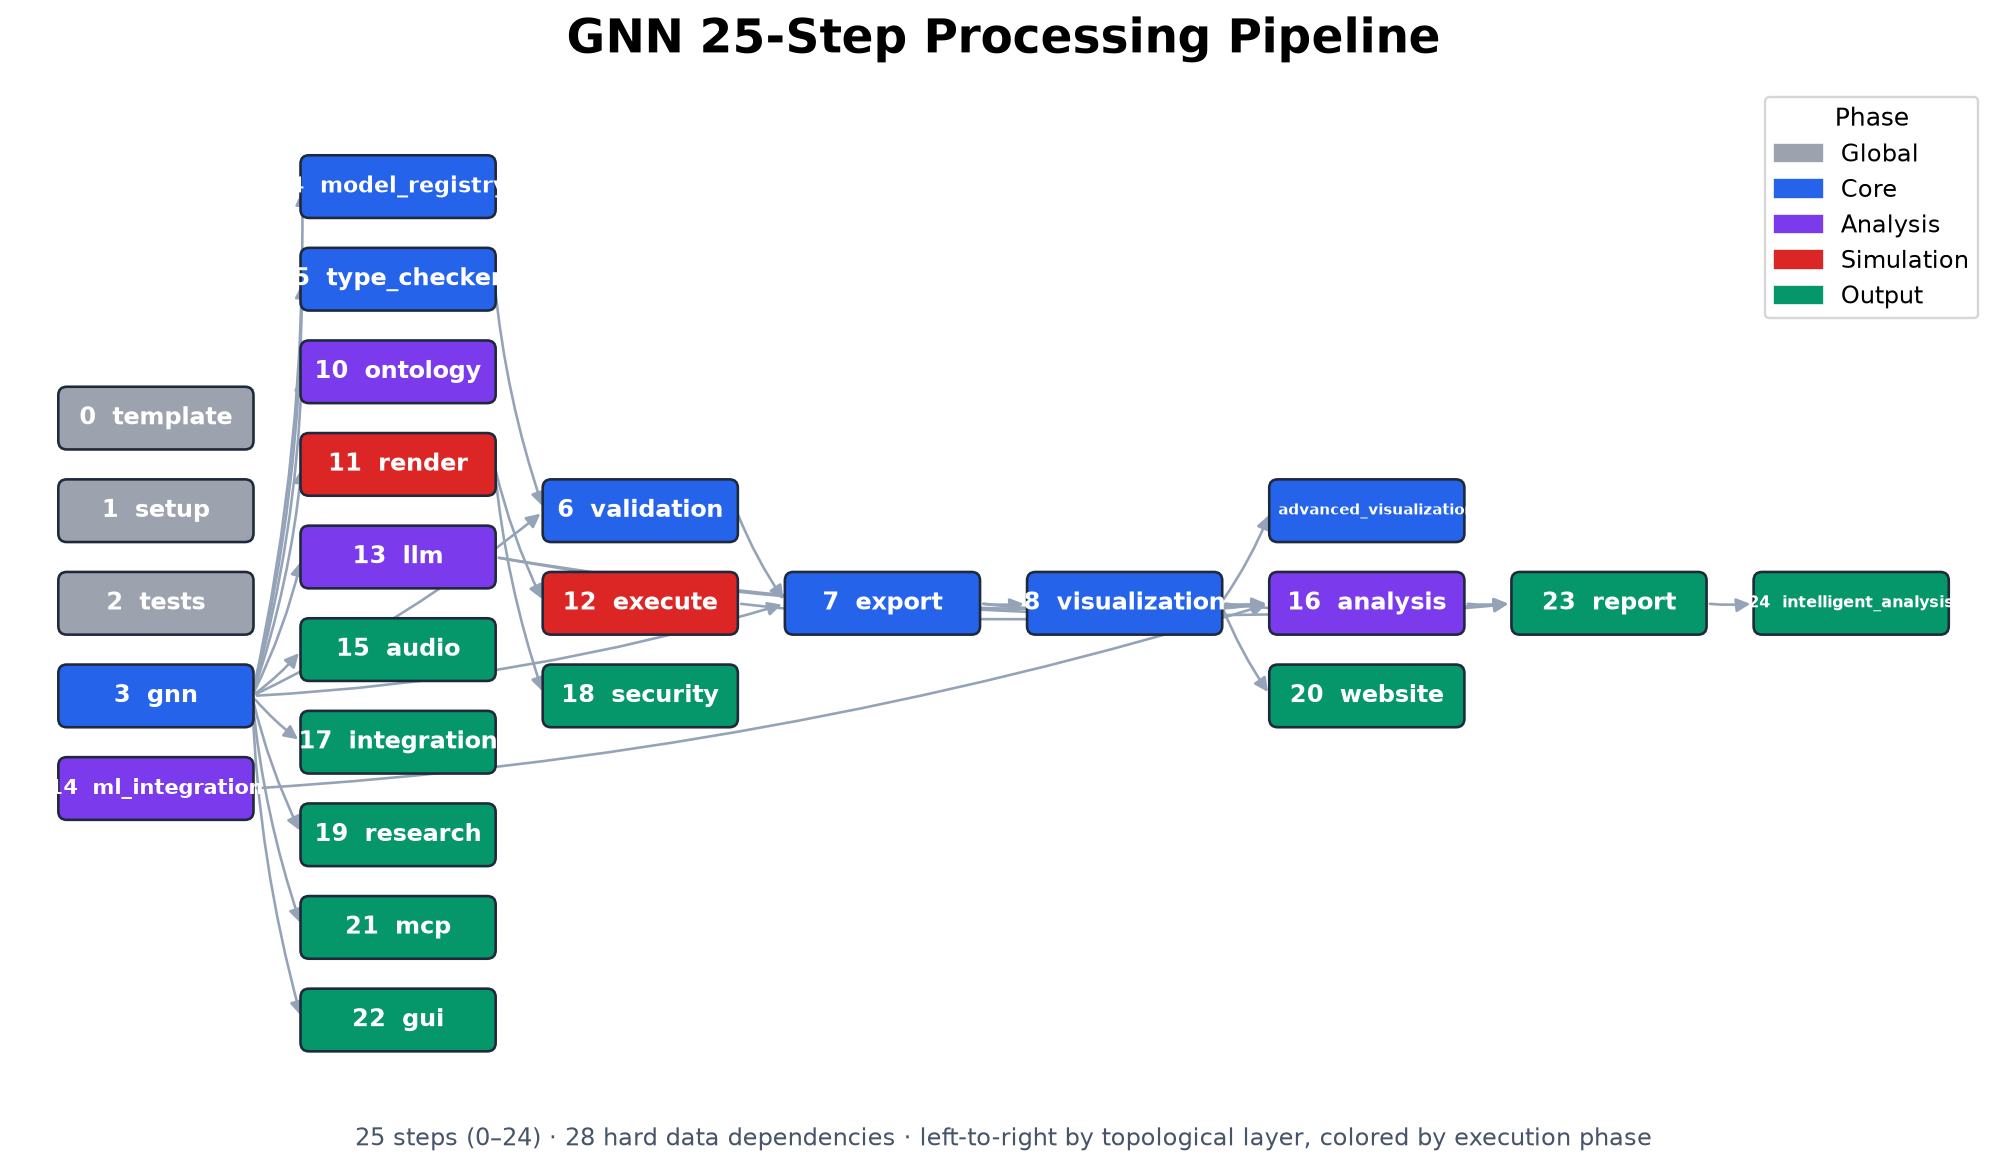
\includegraphics[width=0.9\linewidth,height=0.5\textheight,keepaspectratio,alt={The 25-step GNN processing pipeline as a directed acyclic graph, laid out left to right by topological layer and colored by execution phase (legend, upper right). Each node is the thin step orchestrator under src/gnn/ named in tbl.~; each arrow is a hard data dependency parsed from the Data Dependency Graph block of src/gnn/STEP\_INDEX.md, so any artifact can be traced back to the step that produced it. Parsing (Step 3) fans out to nearly every later step, and analysis (Step 16) collects enrichment from execution, visualization, and the LLM step. The figure is generated from src/gnn/STEP\_INDEX.md at commit 13bd0637c; its footer restates the step count, the number of hard dependencies, and the layout rule.}]{../figures/gnn_pipeline_dag.png}
\caption{The 25-step GNN processing pipeline as a directed acyclic
graph, laid out left to right by topological layer and colored by
execution phase (legend, upper right). Each node is the thin step
orchestrator under \protect\texttt{src/gnn/} named in
tbl.~\ref{tbl:pipeline_steps}; each arrow is a hard data dependency
parsed from the Data Dependency Graph block of
\protect\breaktt{src/gnn/STEP\_INDEX.md}, so any artifact can be traced
back to the step that produced it. Parsing (Step 3) fans out to nearly
every later step, and analysis (Step 16) collects enrichment from
execution, visualization, and the LLM step. The figure is generated from
\protect\breaktt{src/gnn/STEP\_INDEX.md} at commit 13bd0637c; its footer
restates the step count, the number of hard dependencies, and the layout
rule.}\label{fig:pipeline}
\end{figure}

The per-step responsibilities are enumerated in
tbl.~\ref{tbl:pipeline_steps}; each row names a step and the
transformation it owns within the 0--24 range.

\begin{longtable}[]{@{}
  >{\raggedleft\arraybackslash}p{(\linewidth - 4\tabcolsep) * \real{0.4000}}
  >{\raggedright\arraybackslash}p{(\linewidth - 4\tabcolsep) * \real{0.3000}}
  >{\raggedright\arraybackslash}p{(\linewidth - 4\tabcolsep) * \real{0.3000}}@{}}
\caption{The pipeline steps with the thin orchestrator module that owns
each and the one-line purpose parsed from the master table in
\protect\breaktt{src/gnn/STEP\_INDEX.md}. Read the Step column against
the arrows of fig.~\ref{fig:pipeline}: each row's purpose is the
transformation that module owns, and the table is regenerated from the
index at every build, so it cannot drift from the code it
describes.}\label{tbl:pipeline_steps}\tabularnewline
\toprule\noalign{}
\begin{minipage}[b]{\linewidth}\raggedleft
Step
\end{minipage} & \begin{minipage}[b]{\linewidth}\raggedright
Module
\end{minipage} & \begin{minipage}[b]{\linewidth}\raggedright
Purpose
\end{minipage} \\
\midrule\noalign{}
\endfirsthead
\toprule\noalign{}
\begin{minipage}[b]{\linewidth}\raggedleft
Step
\end{minipage} & \begin{minipage}[b]{\linewidth}\raggedright
Module
\end{minipage} & \begin{minipage}[b]{\linewidth}\raggedright
Purpose
\end{minipage} \\
\midrule\noalign{}
\endhead
\bottomrule\noalign{}
\endlastfoot
0 & \texttt{0\_template.py} & Pipeline template \& initialization \\
1 & \texttt{1\_setup.py} & Environment setup \& UV dependency install \\
2 & \texttt{2\_tests.py} & Test suite execution (pytest) \\
3 & \texttt{3\_gnn.py} & GNN file discovery \& multi-format parsing \\
4 & \breaktt{4\_model\_registry.py} & Model versioning \& registry
management \\
5 & \breaktt{5\_type\_checker.py} & GNN type validation \& resource
estimation \\
6 & \texttt{6\_validation.py} & Consistency \& semantic quality
checking \\
7 & \texttt{7\_export.py} & Multi-format export (JSON, XML, GraphML,
GEXF, Pickle) \\
8 & \breaktt{8\_visualization.py} & Graph \& matrix visualization
generation \\
9 & \breaktt{9\_advanced\_viz.py} & Interactive / advanced visualization
(Plotly, D3) \\
10 & \texttt{10\_ontology.py} & Active Inference ontology processing \&
validation \\
11 & \texttt{11\_render.py} & Code generation for simulation
frameworks \\
12 & \texttt{12\_execute.py} & Execute rendered simulation scripts \\
13 & \texttt{13\_llm.py} & LLM-enhanced analysis \& model
interpretation \\
14 & \breaktt{14\_ml\_integration.py} & Machine learning integration \&
model training \\
15 & \texttt{15\_audio.py} & Audio sonification generation (SAPF) \\
16 & \texttt{16\_analysis.py} & Statistical analysis \& cross-simulation
aggregation \\
17 & \breaktt{17\_integration.py} & System integration \& cross-module
coordination \\
18 & \texttt{18\_security.py} & Security validation \& generated code
scanning \\
19 & \texttt{19\_research.py} & Research tools \& literature
references \\
20 & \texttt{20\_website.py} & Static HTML website generation \\
21 & \texttt{21\_mcp.py} & Model Context Protocol processing \& tool
registration \\
22 & \texttt{22\_gui.py} & Interactive GNN constructor GUI \\
23 & \texttt{23\_report.py} & Comprehensive analysis report
generation \\
24 & \breaktt{24\_intelligent\_analysis.py} & AI-powered pipeline
analysis \& executive reports \\
\end{longtable}

This staged design keeps the architecture modular. The implementation is
organized into 44 source packages, one cluster of responsibilities per
concern, and is documented across 624 documentation files so that each
step's contract, inputs, and outputs are specified independently of the
others. New backends or analyses attach to the graph by declaring their
dependencies rather than by editing a monolith, and the deterministic
step ordering means a model processed today yields the same artifacts
when reprocessed tomorrow. The pipeline is kind-agnostic in its plumbing
and kind-aware at its edges: parsing, validation, and export operate on
whatever the file declares, while the rendering and execution steps
consult the classification of sec.~\ref{sec:model_kinds} to decide which
backends a given model can reach and record, explicitly, the ones it
cannot.

\subsection{The Triple Play}\label{the-triple-play}

The reason for separating a single written language from a multi-stage
pipeline is the design goal GNN calls the Triple Play: one model
specification, three coordinated modes of existence. The same GNN text
is simultaneously a human-readable model description, a set of graphical
visualizations of its state space and factor structure, and an
executable cognitive model that can be run as a simulation.
fig.~\ref{fig:triple_play} depicts these three faces and the shared
specification at their center.

\begin{figure}
\centering
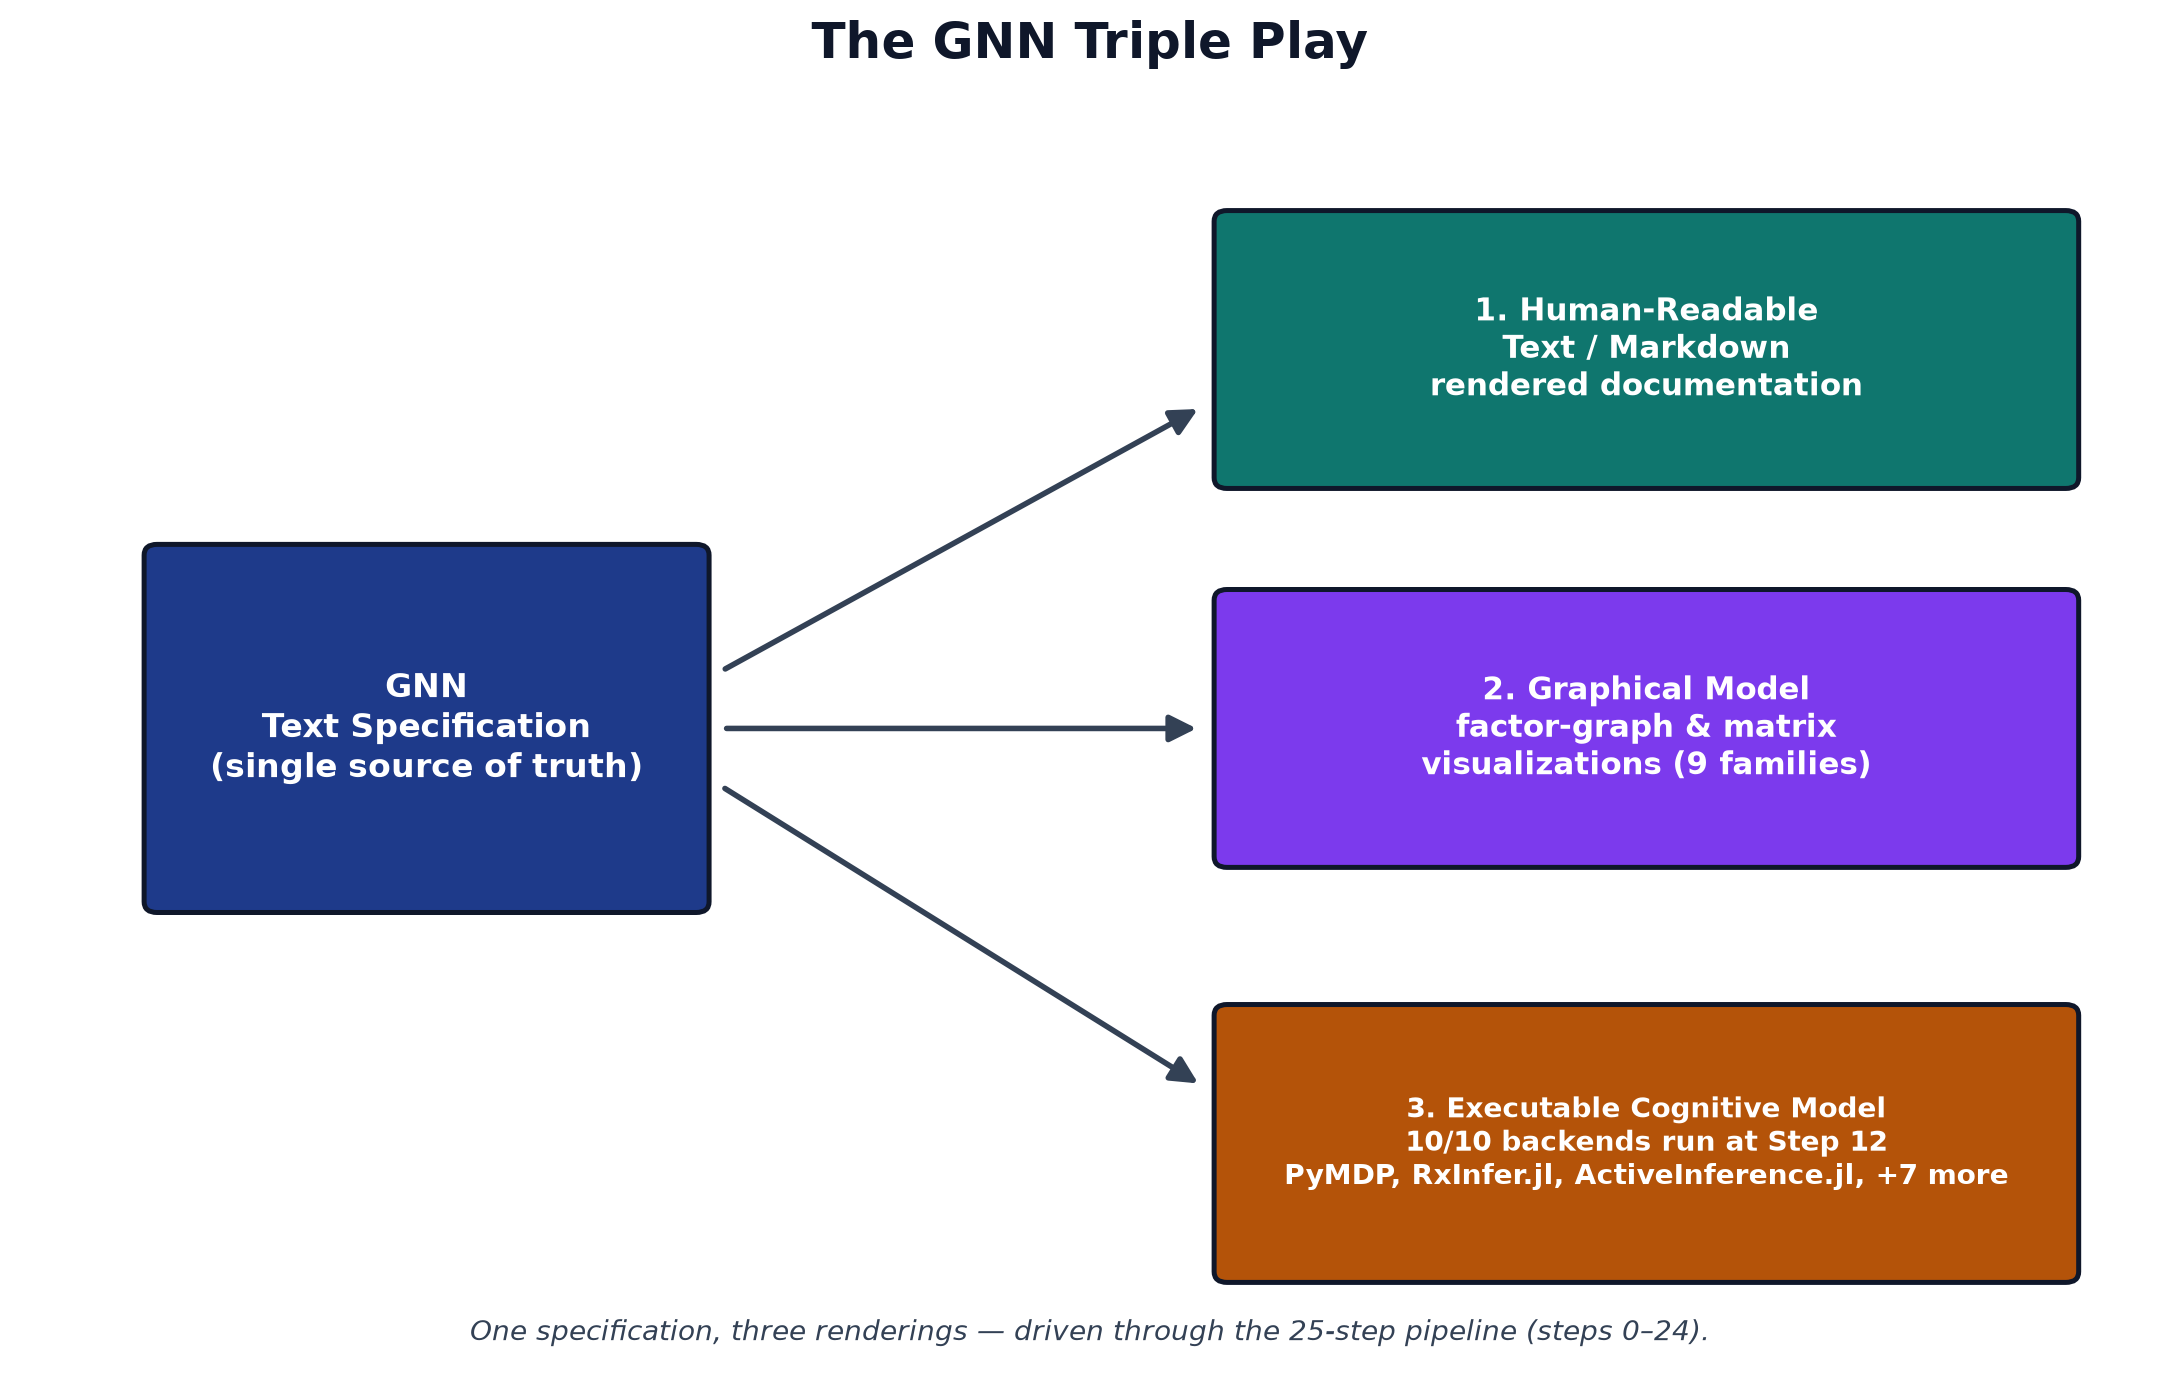
\includegraphics[width=0.7\linewidth,height=0.5\textheight,keepaspectratio,alt={The Triple Play: one GNN text specification (left) and its three coordinated projections (right) --- the human-readable text form, graphical model visualizations, and executable simulation code. All three arrows originate at the same source box because all three projections are generated from one parsed document, which is why they cannot drift apart; the executable node states that 9 of 9 registered backends run at Step 12 and previews three of them by name. Counts are producer tokens at commit 13bd0637c, and the panel is generated by scripts/manuscript\_fig\_triple\_play.py. Take-away: a model is authored once and then read, seen, and run from that single source.}]{../figures/gnn_triple_play.png}
\caption{The Triple Play: one GNN text specification (left) and its
three coordinated projections (right) --- the human-readable text form,
graphical model visualizations, and executable simulation code. All
three arrows originate at the same source box because all three
projections are generated from one parsed document, which is why they
cannot drift apart; the executable node states that 9 of 9 registered
backends run at Step 12 and previews three of them by name. Counts are
producer tokens at commit 13bd0637c, and the panel is generated by
\protect\breaktt{scripts/manuscript\_fig\_triple\_play.py}. Take-away: a
model is authored once and then read, seen, and run from that single
source.}\label{fig:triple_play}
\end{figure}

Each face is generated from the same source, so they cannot drift apart.
The text is the contract a researcher reads and reviews; the
visualizations expose the factor-graph structure for inspection and
communication; and the executable rendering lets the identical model be
simulated across inference frameworks, connecting the written
specification to the discrete message-passing libraries for categorical
Active Inference \citep{heins2022}, to the reactive message-passing and
probabilistic-programming engines that carry the linear-Gaussian kind,
and to the broader tooling ecosystem for compositional model
representation \citep{defelice2021}. Because all three derive from one
parsed document, GNN turns a model from a static artifact into a live
object that can be read, seen, and run without re-encoding it for each
purpose \citep{smith2022}. The Triple Play holds per kind: each of the
three faces is generated from the same classification the pipeline
computed at parse time, so the diagram a reader sees, the notation a
reviewer diffs, and the program a backend executes are all projections
of one declared model kind rather than three loosely coupled guesses
about what the file meant.

\newpage

\section{Methods}\label{sec:methods}

The GeneralizedNotationNotation (GNN) method is realized as a sequence
of deterministic transformations that take a plain-text model
specification and carry it through parsing, validation, code generation,
execution, and reporting. The processing pipeline is organized into 25
numbered steps (steps 0--24), each implemented as a standalone module
with a single responsibility. The methods below describe the path that a
model travels from notation to executable cognitive model and back to
analyzed results, and they state that path per model kind wherever the
kinds part ways: the pipeline's plumbing is kind-agnostic, but rendering
and execution are kind-aware by design. Every quantity reported in this
section is produced from the live repository rather than asserted by
hand; the closing subsection makes that contract explicit.

\subsection{Parsing and Multi-Format
Export}\label{parsing-and-multi-format-export}

The pipeline begins by ingesting GNN model files written in the
plain-text notation. Parsing (step 3) reads each specification, builds
an internal model representation, and re-emits it across a family of
structured export formats so that downstream tools, and human readers,
can consume the same model through whichever serialization they prefer.
The corpus that exercises this stage spans 30 example model files
organized into 11 curated corpora, and it spans the model kinds of
sec.~\ref{sec:model_kinds}: minimal perception fixtures used to test the
parser, discrete categorical agents, continuous linear-Gaussian
state-space models, multi-agent swarms, hierarchical two-level
compositions, and the scaling-study corpus that grows a single family
across state-space sizes. The presence of hierarchical fixtures should
be read as a coverage target, not as a claim that every current backend
fully executes every hierarchical formulation; scaling hierarchical
active inference remains an active research problem in its own right
\citep{rangarajan2026hierarchicalSuccessor}. Treating parsing and export
as a single round-trippable stage means a model authored once becomes
immediately available as a typed object, a normalized text form, and
machine-readable serializations without any manual re-encoding --- and
because the typed object carries the declared matrix vocabulary
verbatim, the kind classification of sec.~\ref{sec:model_kinds} is
computed from the parse result rather than re-derived downstream.

\subsection{Type Checking and
Validation}\label{type-checking-and-validation}

A model that parses is not yet a model that is well-formed. Steps 5 and
6 apply type checking and validation to confirm that the state spaces,
observation modalities, control factors, and the matrices relating them
are mutually consistent before any code is generated. This catches
dimensional mismatches and malformed factor structures at the notation
level, where the diagnostic is cheap and legible, rather than allowing
them to surface as opaque runtime errors deep inside a numerical
backend. Validation is where the kinds receive their shape contracts,
and each kind's contract checks the objects its notation actually
declares.

For a discrete categorical specification, validation reads each declared
\texttt{B} tensor through an orientation diagnostic: the canonical
reading is column-stochastic,
\texttt{B{[}next\_state{]}{[}previous\_state{]}{[}action{]}}, matching
the pymdp convention \citep{heins2022} and the transition semantics
fixed by eq.~\ref{eq:transition}, and the check records every tensor's
detected orientation in its receipt. A row-stochastic textbook literal
--- the transpose of the canonical layout --- is flagged with the
tensor, state factor, and flipped slice indices named, and the opt-in
\texttt{-\/-transpose-b} flag maps such literals onto the canonical
order at load time instead of failing them, recording the transposition
per tensor.

For a continuous linear-Gaussian specification, validation enforces the
Gaussian shape contract of eq.~\ref{eq:lgssm_state} and
eq.~\ref{eq:lgssm_obs}: \texttt{prior\_mean} must carry exactly as many
entries as the latent state, \texttt{Q} and \texttt{prior\_cov} must be
square in the state dimension, and \texttt{R} must be square in the
observation dimension. A covariance whose shape disagrees with the state
or observation declaration is a validation-time diagnostic naming the
mismatched matrix and its dimensions, not a broadcast error inside a
generated script; and the optional closed-loop declarations are checked
as a pair, since a \texttt{goal\_mean} without a \texttt{control\_gain}
(or the reverse) is an incomplete control structure rather than a
passive model.

Validation here is the gate that protects every later stage: rendering,
execution, and analysis all assume a model that has already been
certified consistent for its kind.

\subsection{Rendering to Multiple
Backends}\label{rendering-to-multiple-backends}

The central act of the ``Triple Play'' is turning a validated
specification into executable cognitive models. The rendering stage
emits backend-specific code for 9 registered target frameworks ---
PyMDP, RxInfer.jl, ActiveInference.jl, JAX, DisCoPy, PyTorch, NumPyro,
Stan, bnlearn --- so that a single GNN model can be instantiated as a
simulation in whichever computational ecosystem a researcher already
works in. Each backend is addressed through a registry key that maps the
abstract model onto that framework's idioms for representing generative
models and performing inference. The full mapping from registry key to
backend is given below.

\begin{longtable}[]{@{}lll@{}}
\caption{Render targets declared in
\protect\breaktt{src/gnn/render/framework\_registry.py}, one row per
registry key in registry order. The \emph{Executes} column is the
registry's own \protect\breaktt{supports\_execution} flag: 9 of 9
backends have a Step-12 executor, and a \protect\texttt{render-only}
entry would mean generated code with no Step-12 executor. Read this
table against tbl.~\ref{tbl:model_families}, which shows which families
actually target each
backend.}\label{tbl:backend_registry}\tabularnewline
\toprule\noalign{}
Registry key & Backend & Executes \\
\midrule\noalign{}
\endfirsthead
\toprule\noalign{}
Registry key & Backend & Executes \\
\midrule\noalign{}
\endhead
\bottomrule\noalign{}
\endlastfoot
\texttt{pymdp} & PyMDP & yes \\
\texttt{rxinfer} & RxInfer.jl & yes \\
\breaktt{activeinference\_jl} & ActiveInference.jl & yes \\
\texttt{jax} & JAX & yes \\
\texttt{discopy} & DisCoPy & yes \\
\texttt{pytorch} & PyTorch & yes \\
\texttt{numpyro} & NumPyro & yes \\
\texttt{stan} & Stan & yes \\
\texttt{bnlearn} & bnlearn & yes \\
\end{longtable}

Because rendering is kind-aware, the registry is best read as a
capability matrix rather than a flat list: which backends can render a
discrete categorical model, which can render a continuous
linear-Gaussian model, and which of them execute at Step 12. That
per-framework, per-kind view is auto-injected below.

\begin{longtable}[]{@{}llll@{}}
\caption{Model kinds each render framework supports, read entirely from
the flags in \protect\breaktt{src/gnn/render/framework\_registry.py} ---
the same source as tbl.~\ref{tbl:backend_registry}. A continuous cell of
\protect\texttt{unsupported} is the renderer's own status for
continuous-state models; a render-only entry has no Step-12 executor.
Read with tbl.~\ref{tbl:model_kinds}, which groups the same flags by
model kind.}\label{tbl:framework_capability}\tabularnewline
\toprule\noalign{}
Framework & Discrete render & Continuous render & Executor status \\
\midrule\noalign{}
\endfirsthead
\toprule\noalign{}
Framework & Discrete render & Continuous render & Executor status \\
\midrule\noalign{}
\endhead
\bottomrule\noalign{}
\endlastfoot
PyMDP & yes & unsupported & executor \\
RxInfer.jl & yes & yes & executor \\
ActiveInference.jl & yes & unsupported & executor \\
JAX & yes & yes & executor \\
DisCoPy & yes & unsupported & executor \\
PyTorch & yes & yes & executor \\
NumPyro & yes & yes & executor \\
Stan & yes & yes & executor \\
bnlearn & yes & unsupported & executor \\
\end{longtable}

The registry surface of these backends --- registry key, display name,
implementation language, and which of them the cross-framework gate
compares --- is summarized in fig.~\ref{fig:backend_matrix}; the
family-by-backend coverage itself is shown in
fig.~\ref{fig:family_matrix}.

\begin{figure}
\centering
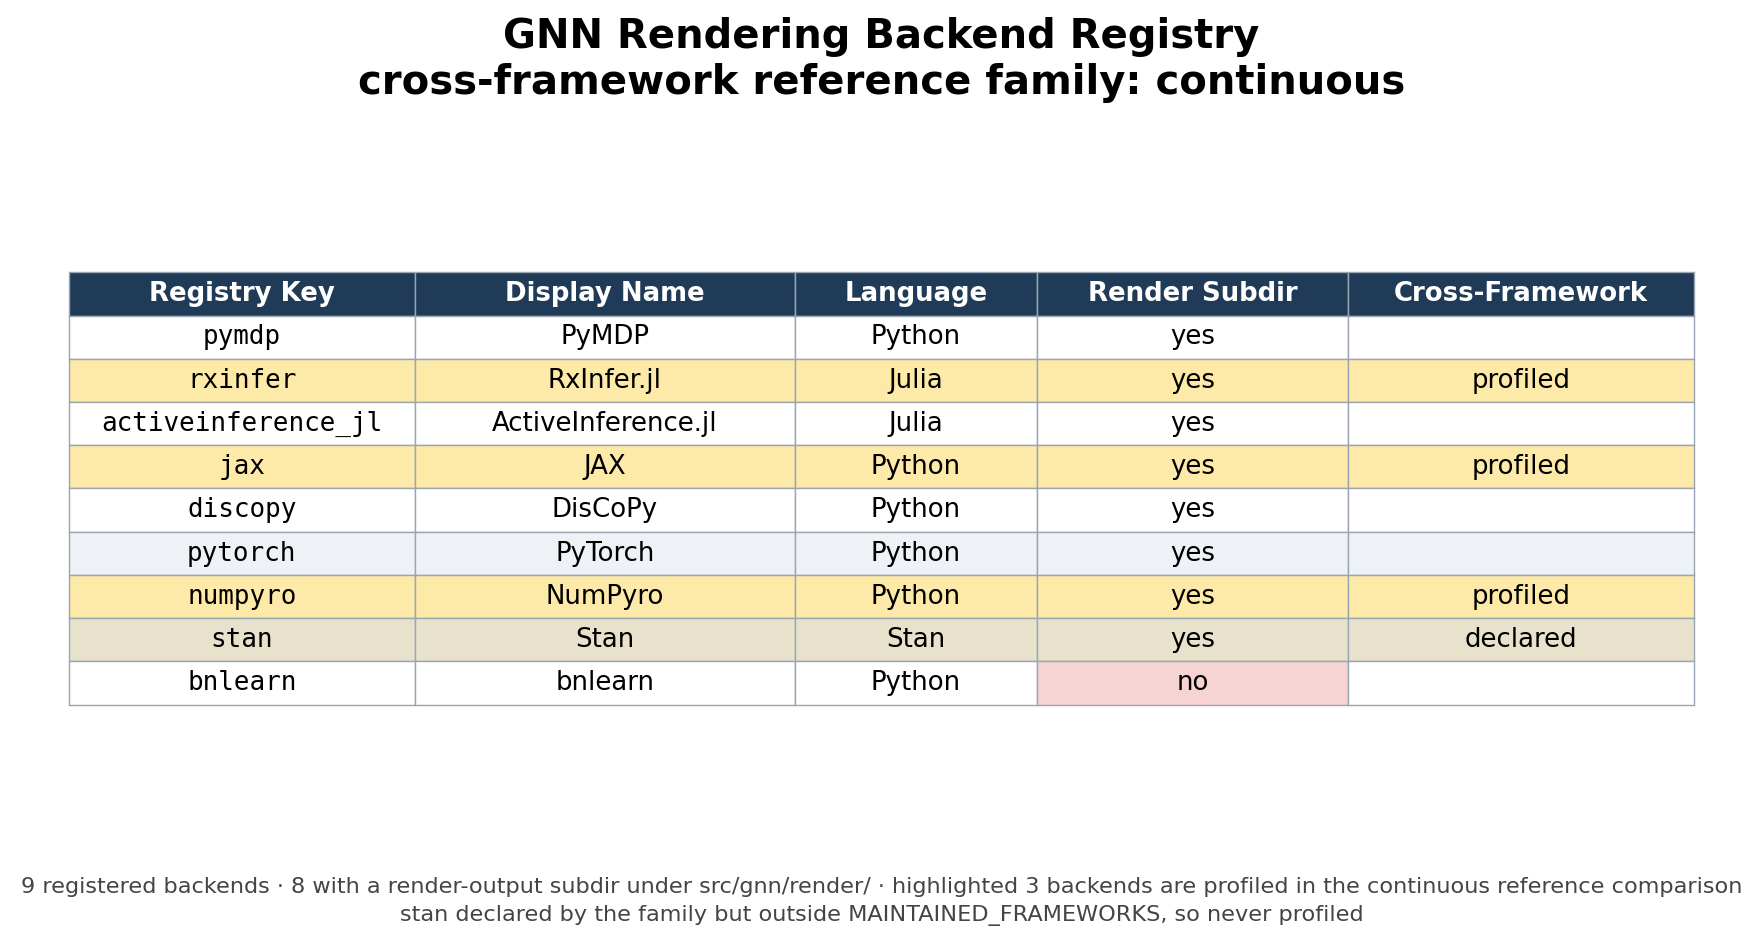
\includegraphics[width=0.85\linewidth,height=0.5\textheight,keepaspectratio,alt={The GNN rendering backend registry as a table: one row per registered backend, with its registry key, display name, implementation language, whether a render-output subdirectory exists under src/gnn/render/, and its role in the cross-framework reference comparison. Amber rows are the backends the reliability gate profiles for the continuous family; the tan row (Stan) is declared by that family but sits outside the maintained set, so it is never profiled; a red Render-Subdir cell would mean a registry entry with no subdirectory. The table is read directly from src/gnn/render/framework\_registry.py and the model-family manifest at commit 13bd0637c, and its footer summarizes the row counts. Take-away: registration, render presence, and profiling status are three different claims, and the table keeps them apart.}]{../figures/gnn_backend_capability_matrix.png}
\caption{The GNN rendering backend registry as a table: one row per
registered backend, with its registry key, display name, implementation
language, whether a render-output subdirectory exists under
\protect\texttt{src/gnn/render/}, and its role in the cross-framework
reference comparison. Amber rows are the backends the reliability gate
profiles for the continuous family; the tan row (Stan) is declared by
that family but sits outside the maintained set, so it is never
profiled; a red Render-Subdir cell would mean a registry entry with no
subdirectory. The table is read directly from
\protect\breaktt{src/gnn/render/framework\_registry.py} and the
model-family manifest at commit 13bd0637c, and its footer summarizes the
row counts. Take-away: registration, render presence, and profiling
status are three different claims, and the table keeps them
apart.}\label{fig:backend_matrix}
\end{figure}

\subsubsection{Rendering by Model Kind}\label{rendering-by-model-kind}

\textbf{Discrete categorical models} are the fully supported case: every
registered backend declares the categorical POMDP vocabulary --- the
\texttt{A}, \texttt{B}, \texttt{C}, \texttt{D} matrices required and
\texttt{E} optional --- so the renderer can emit idiomatic code for all
of them, and the cross-framework reference comparison of
sec.~\ref{sec:artifacts_evidence} anchors on exactly this breadth.

\textbf{Continuous linear-Gaussian models} take the native paths built
for them. The RxInfer.jl renderer carries dedicated continuous
strategies that emit reactive message-passing code over the Gaussian
state-space model; the JAX, PyTorch, and NumPyro renderers generate
standalone scripts that filter the belief state numerically --- and,
when the closed-loop declarations of eq.~\ref{eq:closed_loop} are
present, steer it toward the preferred state --- with the JAX lane
enabling 64-bit precision for the covariance arithmetic; and the Stan
renderer emits the model as a probabilistic program. The
categorical-only backends --- pymdp, ActiveInference.jl, DisCoPy, and
bnlearn --- do not fabricate a translation: each reports the continuous
model as \texttt{unsupported}, with a recorded reason, and the status is
counted under unsupported framework renderings rather than as a failure
--- never rendered, never executed, and excluded from the success
denominator so the run's rate measures the backends that could actually
attempt the model. DisCoPy's boundary is representative: its translator
draws categorical POMDP string diagrams and has no linear-Gaussian
diagram semantics, so a continuous model is reported unsupported rather
than drawn as a discrete stand-in.

\textbf{Composed kinds} render through their substrate. A multi-agent
model renders along the discrete path, with the per-agent matrix
declarations mapped to per-agent structures in the target framework; a
hierarchical model renders either composed --- the per-level matrices
composed into one joint POMDP for the categorical backends --- or
natively, through the RxInfer.jl two-level strategies; a
parameter-learning model renders through the strategy layer that emits
joint variational message-passing code for its Dirichlet-declared
matrix; and the remaining structural shapes dispatch to their own
strategy modules rather than to special cases scattered through the
renderers.

\textbf{Structural wrappers} have no renderable form at all: they
declare boundary structure only, with neither a categorical nor a
continuous parameterization, so every framework reports them
\texttt{unsupported} upstream with the structural-spec reason rather
than silently rendering them as a discrete stand-in that would fail on
missing matrices. The status is the design working, not a defect: a
wrapper is an interface statement, and the pipeline's response is to say
so in every receipt rather than to guess a model body the author never
declared.

By generating code rather than asking authors to port models by hand,
the method keeps a single source of truth in the notation while still
reaching the discrete message-passing libraries \citep{heins2022},
reactive message-passing lineage
\citep{bagaev2021reactiveMessagePassing}, and categorical, diagrammatic
frameworks \citep{defelice2021} that different research communities have
built. The underlying mathematics that compatible backends share ---
inference over the generative model the notation declares, whether that
is categorical free-energy minimization \citep{dacosta2020, smith2022}
or Gaussian filtering and control --- is the common substrate the
renderer attempts to preserve; where a backend cannot express a kind
faithfully, GNN records that boundary as an explicit unsupported status
rather than treating all registered backends as equivalent.

\subsection{Execution}\label{execution}

\subsubsection{Executing by Model Kind}\label{executing-by-model-kind}

Generated backend code is not left as a static artifact. The execution
stage (step 12) runs the rendered models, driving the inference and
behavior that the notation describes and producing concrete traces,
beliefs, and outputs. All 9 registered backends --- PyMDP, RxInfer.jl,
ActiveInference.jl, JAX, DisCoPy, PyTorch, NumPyro, Stan, bnlearn ---
have an executor at this step, and execution is kind-aware in the same
sense rendering is: a backend executes the models its renderer can
express, and records an explicit status for the ones it cannot.

\textbf{Discrete executors} run the categorical models end to end, and
they guard their own runtime assumptions: the generated pymdp scripts,
for example, sanity-check the installed library for the current Agent
interface at startup and exit fast with a clear message when an
unsupported wheel is present, so a stale environment produces a legible
diagnostic instead of a mysterious failure deep in a simulation loop.

\textbf{Continuous executors} run the generated standalone scripts over
the Gaussian state-space model --- filtering to a posterior, and with
the closed-loop declarations in place, closing the control loop on
beliefs --- so a continuous model produces traces on the same terms as a
discrete one, on the backends that carry the kind.

\textbf{Generator-backed and render-adjacent lanes} extend execution
beyond the registry's render paths. The bnlearn lane is
generator-backed: it renders a runnable Python program from the same
parsed model the other lanes consume, and it skips with a recorded
status when the \texttt{bnlearn} package is absent, so a lean checkout
degrades explicitly rather than failing. A separate execute-side bridge
verifies rendered Lean documents against the fep\_lean bridge contract,
which is how the notation reaches a proof assistant without a
render-registry entry. Skipped, degraded, and unsupported lanes are
recorded as explicit statuses in the cross-framework comparison rather
than silently omitted.

This closes the loop from text to running cognitive model: the same
specification that was type-checked and exported is now exercised
numerically, so that claims about a model's behavior rest on having
actually run it rather than on inspection of the source alone.

\subsection{Long-Running Orchestration
Contracts}\label{long-running-orchestration-contracts}

GNN 3.0.0 extended the pipeline with three safe-by-design orchestration
contracts that let an extended run be observed, paused, resumed, and
audited without ever mutating live infrastructure. \emph{Durable
observation streams} record file- and array-backed stream manifests with
content checksums and replayable execution traces, so that a long run
can be re-derived deterministically before any live sensor or
device-backed stream is introduced. \emph{Resumable run sessions} carry
run-session manifests with atomic checkpoint and resume, status
inspection, and cancellation-safe cleanup, so that an extended
model-family acceptance run can be interrupted and resumed without
corrupting partial state. \emph{Auditable container plans} generate
hardened container plans together with an explicit static security
review and a rollback descriptor, deliberately stopping short of
touching any real cluster. Each contract only generates and validates
data; none performs live mutation, and each is governed by a strict
acceptance gate and exercised through dedicated Model Context Protocol
tools. fig.~\ref{fig:orchestration} shows how the three contracts
compose into one inspectable orchestration surface.

\begin{figure}
\centering
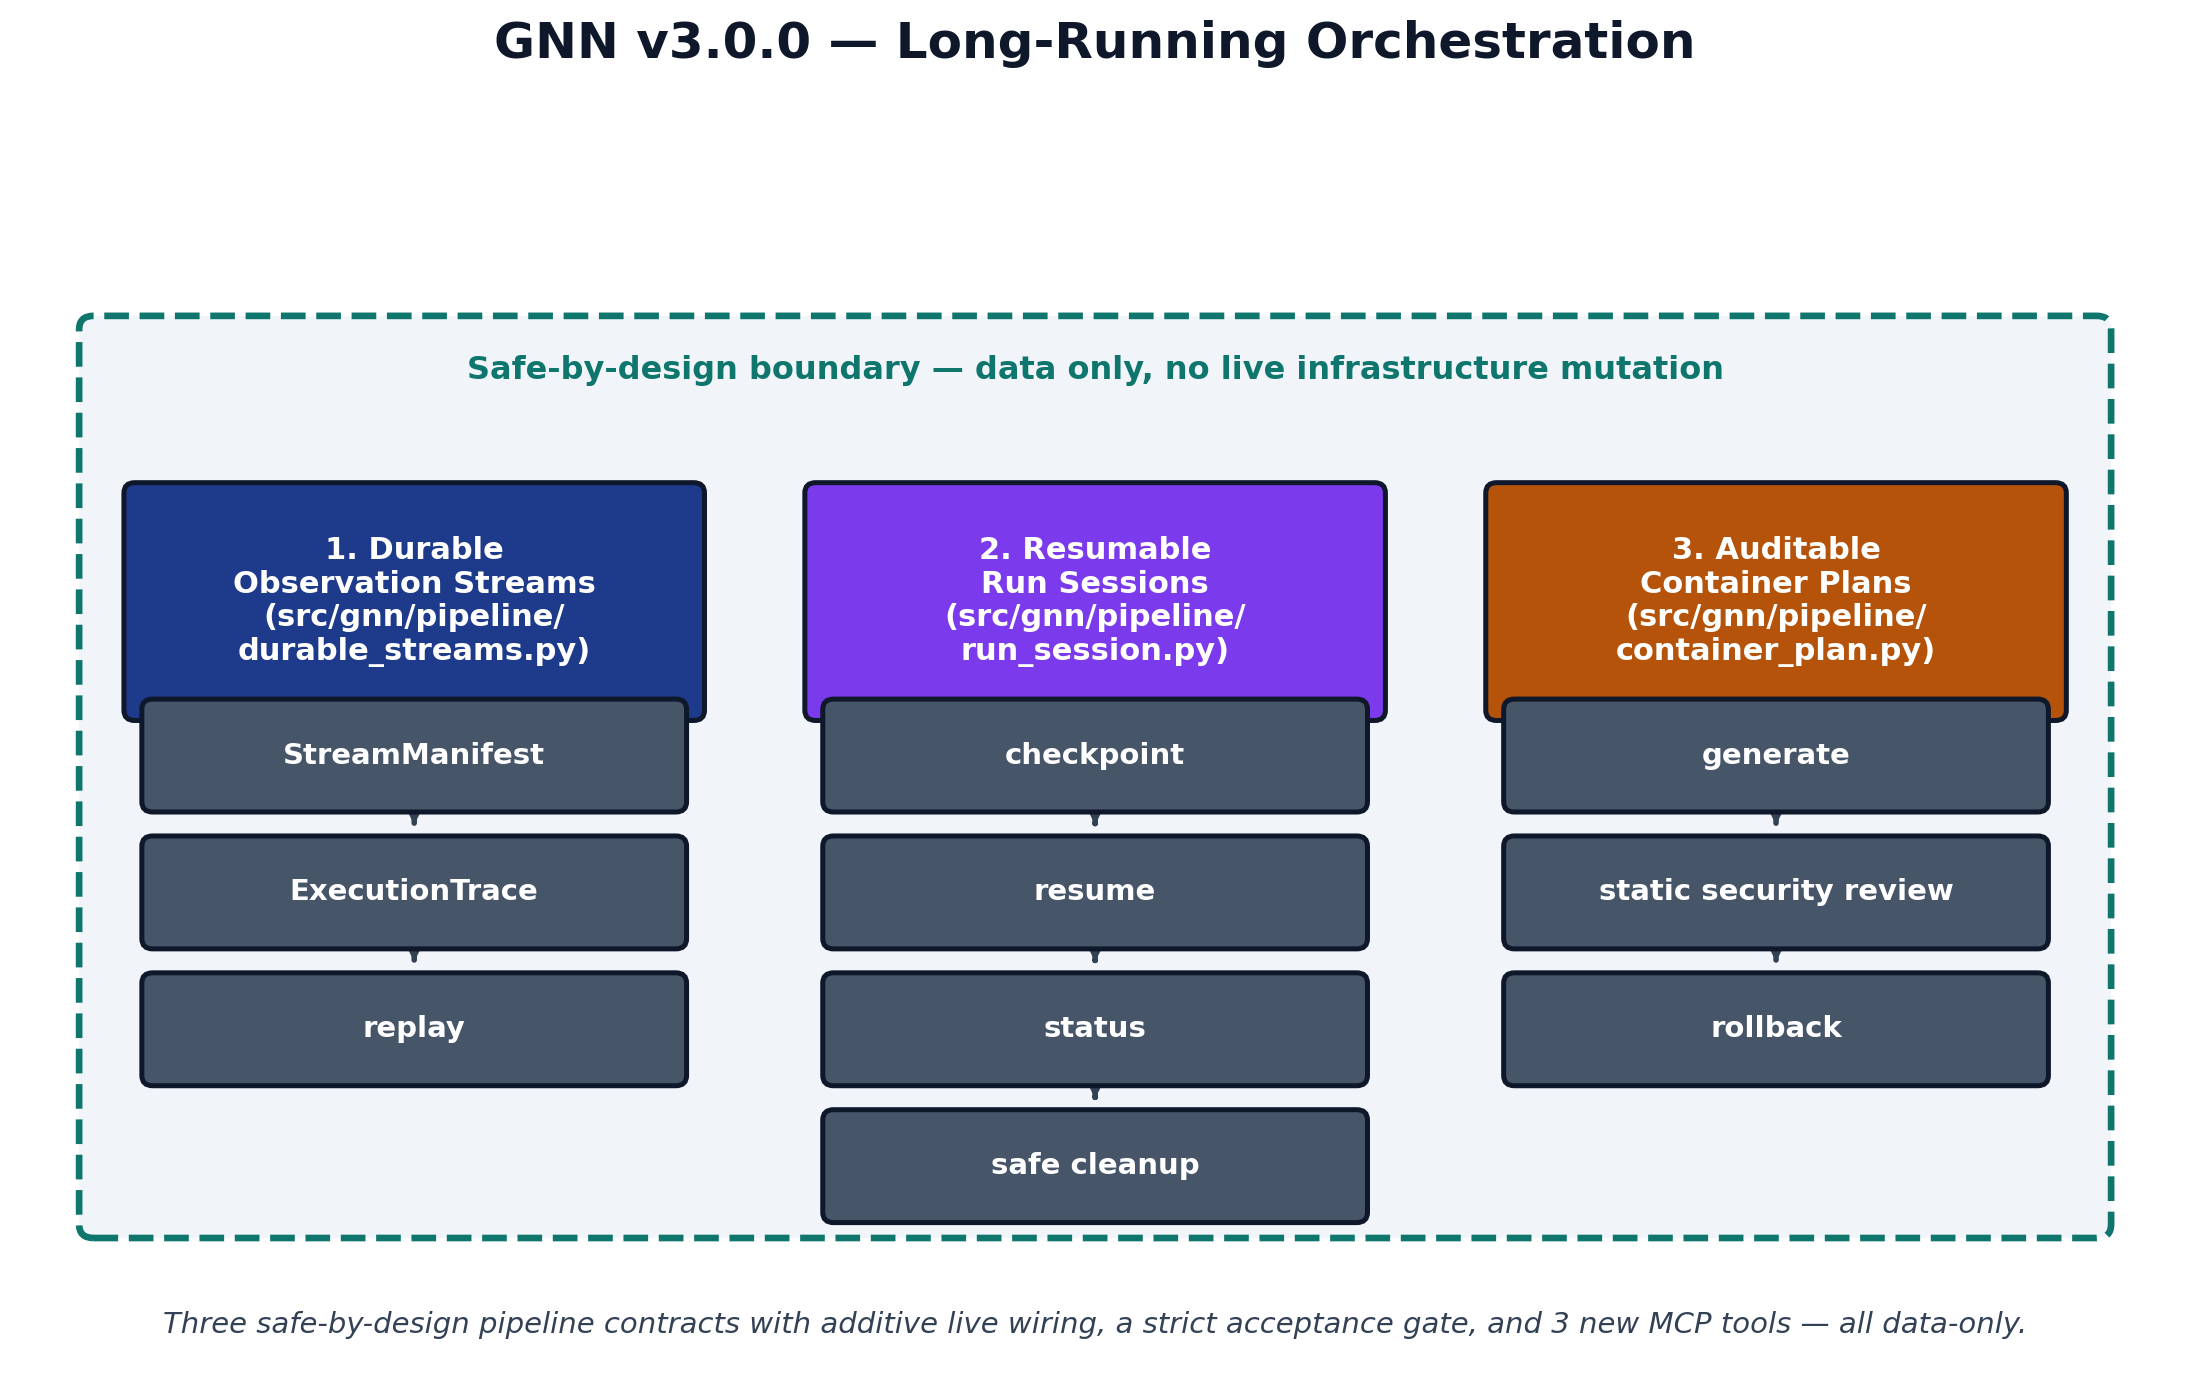
\includegraphics[width=0.85\linewidth,height=0.5\textheight,keepaspectratio,alt={The three safe-by-design orchestration contracts introduced in GNN 3.0.0, side by side inside the dashed boundary that states their shared invariant: generate and validate data only, never mutate live infrastructure. Each column names the contract's source module under src/gnn/pipeline/ and chains its stages top to bottom --- StreamManifest, ExecutionTrace, and replay for durable observation streams; checkpoint, resume, status, and safe cleanup for resumable run sessions; generate, static security review, and rollback for container plans. Arrows give the order the stages run in, and nothing exits the boundary. The panel is a fixed-layout drawing of the three contracts; the acceptance gates and the Model Context Protocol tools that exercise them are described in the text above. Take-away: long-running orchestration gains capability only as fast as it becomes inspectable.}]{../figures/gnn_orchestration.png}
\caption{The three safe-by-design orchestration contracts introduced in
GNN 3.0.0, side by side inside the dashed boundary that states their
shared invariant: generate and validate data only, never mutate live
infrastructure. Each column names the contract's source module under
\protect\breaktt{src/gnn/pipeline/} and chains its stages top to bottom
--- StreamManifest, ExecutionTrace, and replay for durable observation
streams; checkpoint, resume, status, and safe cleanup for resumable run
sessions; generate, static security review, and rollback for container
plans. Arrows give the order the stages run in, and nothing exits the
boundary. The panel is a fixed-layout drawing of the three contracts;
the acceptance gates and the Model Context Protocol tools that exercise
them are described in the text above. Take-away: long-running
orchestration gains capability only as fast as it becomes
inspectable.}\label{fig:orchestration}
\end{figure}

\subsection{Analysis, Visualization, and
Reporting}\label{analysis-visualization-and-reporting}

The final group of stages turns execution results into interpretable
evidence. Analysis (step 16) processes the outputs of execution into
structured findings; visualization (step 8) and the rendering of figures
(step 9) translate model structure and results into graphical form,
supporting the graphical leg of the Triple Play; and the reporting stage
(step 23) assembles these artifacts into a coherent summary of what the
model is and how it behaved. Because each stage writes its outputs to a
known location, the chain from a notation file to a finished report is
fully traceable, and any figure or number in a report can be followed
back to the step and model that produced it. Analysis reads the per-kind
rendering and execution receipts as well: a continuous model whose
categorical-only lanes report \texttt{unsupported} yields a different
evidence profile than one whose continuous-capable lanes failed, and the
reports keep those situations apart.

\subsection{Reproducibility and
Auto-Injection}\label{reproducibility-and-auto-injection}

Every count reported in this manuscript is emitted by the producer
\breaktt{scripts/z\_generate\_manuscript\_variables.py} from the
repository state at commit 13bd0637c, not typed by hand. The producer
reads that commit's source surfaces directly --- the step modules, the
source tree, the model-family manifest, and the framework registry ---
together with the project's maintained ledgers, notably the Model
Context Protocol tool audit (\breaktt{src/gnn/mcp/audit\_report.json},
itself regenerated by the test suite). From these it emits a manifest of
named tokens --- counts of pipeline steps and their modules, source
packages and files, model families, backends, example files partitioned
by model kind, tests, and tools --- plus the two capability tables this
manuscript injects: the model-kind table (tbl.~\ref{tbl:model_kinds})
and the framework capability matrix
(tbl.~\ref{tbl:framework_capability}). The renderer substitutes the
tokens into the prose at build time. Filesystem-derived counts are
recomputed on every run; ledger-derived counts (such as the backend
registry) are re-read from a fixed repository state, so a fixed
repository state yields the same values, and authors are prohibited from
hard-coding any number that has a corresponding token. This makes the
manuscript a faithful, regenerable description of the system it
documents: when the 25-step pipeline, the 9 rendering backends, or the
30-file example corpus change --- or when the discrete-to-continuous
exemplar balance shifts --- the reported numbers change with them on the
next build, and \breaktt{scripts/check\_manuscript\_tokens.py} fails the
build if a section reintroduces a literal that a token already owns.

\newpage

\section{Artifacts and Evidence}\label{sec:artifacts_evidence}

This section reports what the project has actually produced and how each
quantitative claim is grounded. Every number below is substituted at
render time from the deterministic producer, which reads the repository
state at commit 13bd0637c, so each figure here is regenerated from the
artifacts it describes rather than transcribed.

\subsection{Model-Family Coverage}\label{model-family-coverage}

GNN ships a curated corpus of model families that exercise the language
across the difficulty gradient from minimal parser fixtures to full
multi-agent and scaling studies. The manifest registers 9 families
(basics, discrete, continuous, hierarchical, multiagent, precision,
structured, gridworld, scaling-study) across 9 target directories, and
\texttt{input/gnn\_files} holds 11 corpus directories containing 30
concrete example models. The three sets are not coextensive, and the
manuscript does not treat them as one. Registered in no family:
\breaktt{input/gnn\_files/learning}, \breaktt{input/gnn\_files/recursive}
(2 of the 11 corpus directories), covered in
sec.~\ref{sec:limitations_next_steps}. Registered but outside the
scanned tree: none, because all 9 target directories are themselves
\texttt{input/gnn\_files} corpus directories. Each family declares the
simulation frameworks it is meant to drive, which is what lets the same
text model fan out across the executable-model leg of the Triple Play
\citep{gnn2023}. The families and their declared frameworks are
enumerated below.

The exemplar corpus partitions cleanly by model kind, and the partition
is itself a token: 27 of the 30 example specifications are
discrete-state --- the discrete categorical kind and its composed
variants --- and 3 are continuous linear-Gaussian specifications in the
continuous family folder. The cold-start index
\breaktt{input/gnn\_files/INDEX.md} catalogues every exemplar with its
kind, its task folder, and a suggested reading order, and is the fastest
surface for a reader who wants to move from this prose to a runnable
file of a given kind.

The per-kind evidence is generated, not asserted: families that declare
a capability axis (the continuous family declares the continuous-render
axis) carry a backend split in tbl.~\ref{tbl:model_families} that is
generated from the registry's own capability flags, so the table cannot
disagree with the code that decides renderability. Reading the ledgers
by kind is therefore mechanical --- a continuous-family receipt shows
the continuous-capable backends attempted and the categorical-only
backends recorded \texttt{unsupported}, while a discrete-family receipt
shows the categorical breadth the cross-framework gate anchors on
(tbl.~\ref{tbl:framework_capability} is the per-kind key).

\begin{longtable}[]{@{}
  >{\raggedright\arraybackslash}p{(\linewidth - 4\tabcolsep) * \real{0.3333}}
  >{\raggedright\arraybackslash}p{(\linewidth - 4\tabcolsep) * \real{0.3333}}
  >{\raggedright\arraybackslash}p{(\linewidth - 4\tabcolsep) * \real{0.3333}}@{}}
\caption{Model families declared in
\protect\breaktt{input/model\_family\_manifest.json} with the simulation
frameworks each family targets and a generated description. The
\emph{Frameworks} column is the family's declared targets, verbatim from
the manifest; the capability splits appended to some descriptions are
generated from \protect\breaktt{src/gnn/render/framework\_registry.py}
flags, not authored in the manifest, so they cannot disagree with the
registry. Read with tbl.~\ref{tbl:backend_registry} (what each backend
is) and fig.~\ref{fig:family_matrix} (the same coverage as a
matrix).}\label{tbl:model_families}\tabularnewline
\toprule\noalign{}
\begin{minipage}[b]{\linewidth}\raggedright
Family
\end{minipage} & \begin{minipage}[b]{\linewidth}\raggedright
Frameworks
\end{minipage} & \begin{minipage}[b]{\linewidth}\raggedright
Description
\end{minipage} \\
\midrule\noalign{}
\endfirsthead
\toprule\noalign{}
\begin{minipage}[b]{\linewidth}\raggedright
Family
\end{minipage} & \begin{minipage}[b]{\linewidth}\raggedright
Frameworks
\end{minipage} & \begin{minipage}[b]{\linewidth}\raggedright
Description
\end{minipage} \\
\midrule\noalign{}
\endhead
\bottomrule\noalign{}
\endlastfoot
\texttt{basics} & pymdp & Minimal perception fixtures used for parser
and validator smoke coverage. \\
\texttt{discrete} & pymdp & Discrete POMDP and HMM-style active
inference fixtures. \\
\texttt{continuous} & jax, numpyro, stan, rxinfer & Continuous-state
linear-Gaussian fixtures (F/H/Q/R + Gaussian prior;
continuous\_navigation closes the loop on beliefs). Native on
RxInfer.jl, JAX, PyTorch, NumPyro, Stan; reported unsupported (not
failed) on PyMDP, ActiveInference.jl, DisCoPy, bnlearn. \\
\texttt{hierarchical} & pymdp, rxinfer, jax & Hierarchical and temporal
model fixtures (per-level matrices composed into a joint POMDP for
categorical backends; RxInfer.jl renders two-level models natively). \\
\texttt{multiagent} & rxinfer & Multi-agent coordination and swarm
fixtures. \\
\texttt{precision} & pymdp & Precision weighting and curiosity-driven
fixtures. \\
\texttt{structured} & pymdp & Structured factor graph and posterior
fixtures. \\
\texttt{gridworld} & pymdp, rxinfer, activeinference\_jl & Gridworld
POMDP fixture used for cross-framework acceptance checks. \\
\texttt{scaling-study} & pymdp & PyMDP scaling-study fixtures, sampled
conservatively for acceptance. \\
\end{longtable}

The family-by-framework structure is shown in
fig.~\ref{fig:family_matrix}, which renders the coverage matrix directly
from the family registry rather than from a hand-maintained table.

\begin{figure}
\centering
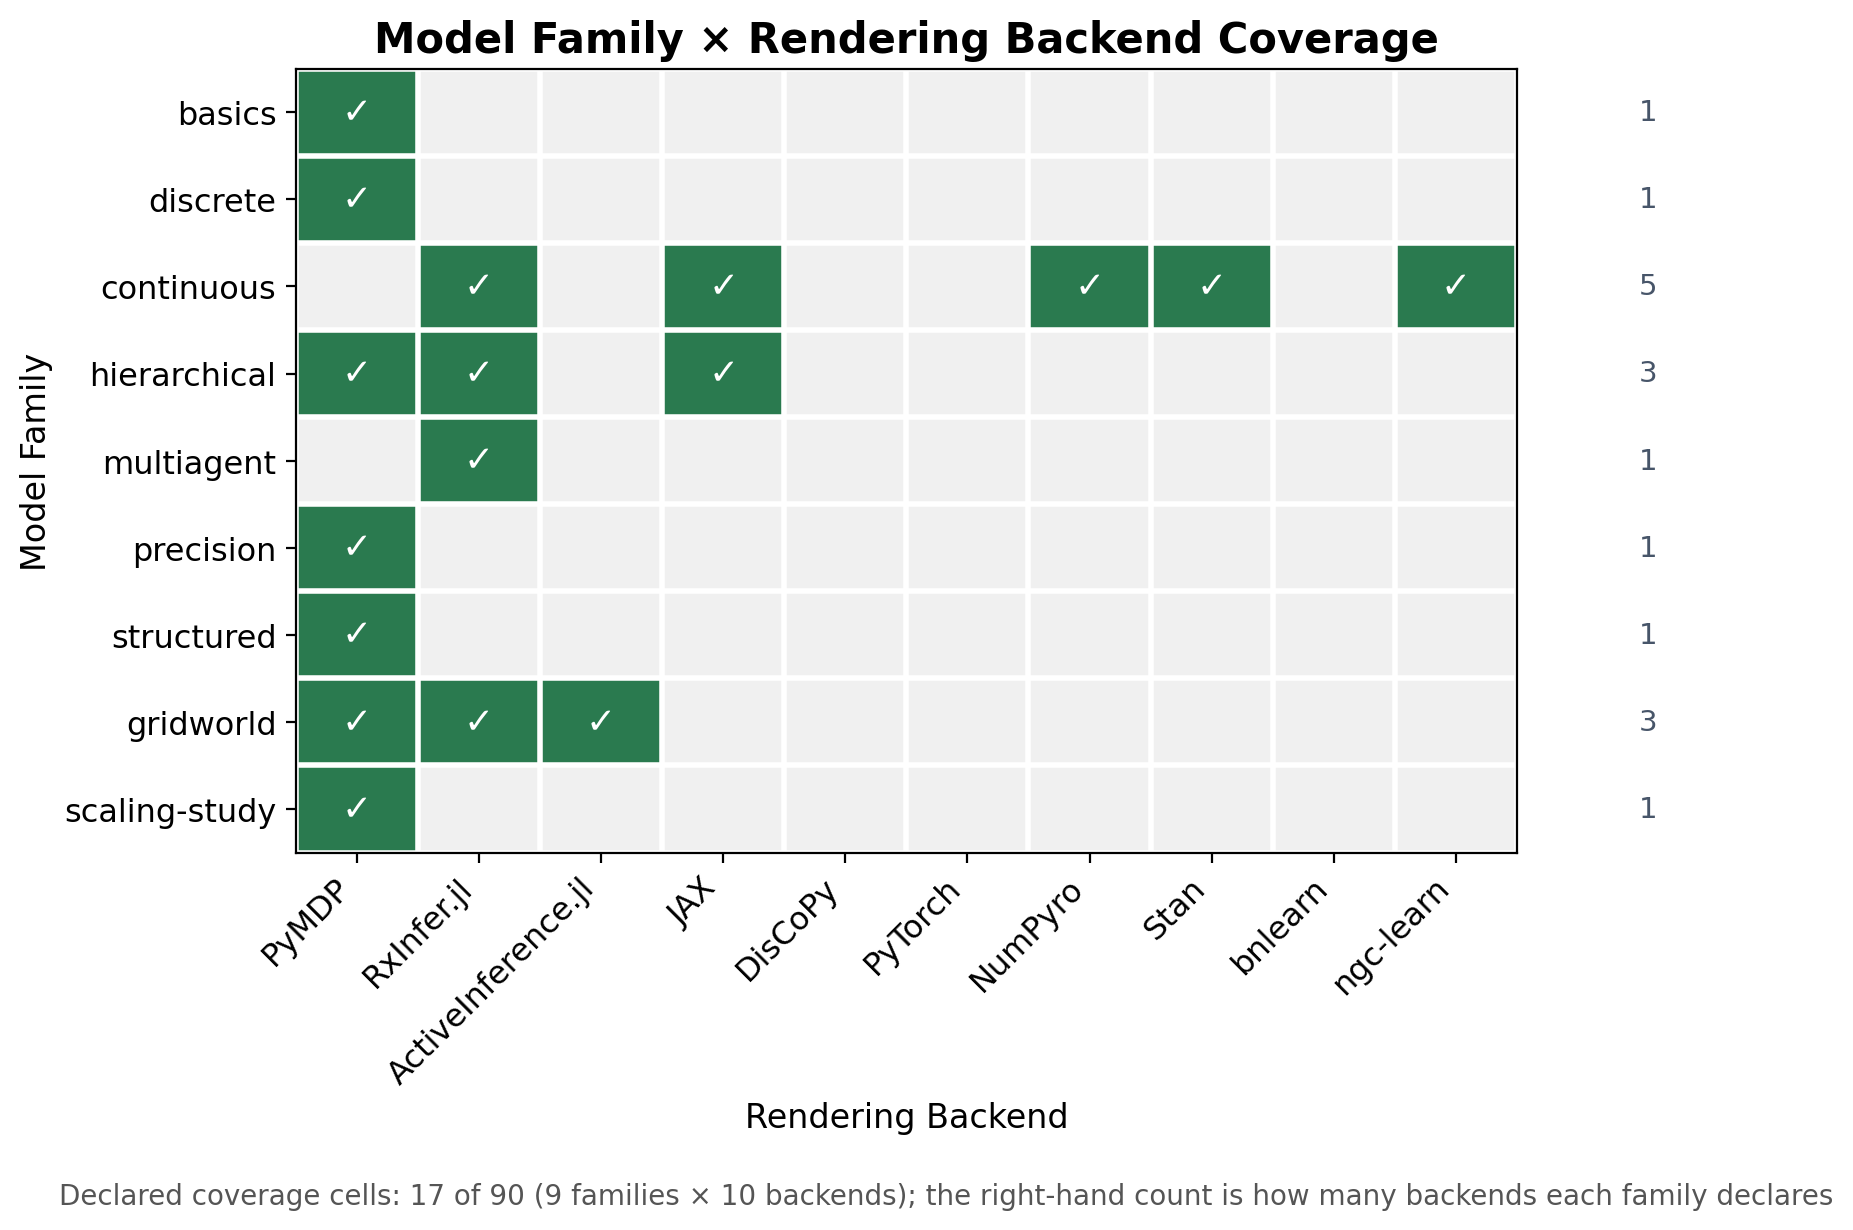
\includegraphics[width=0.85\linewidth,height=0.5\textheight,keepaspectratio,alt={Model-family coverage across the registered rendering backends: one row per family from input/model\_family\_manifest.json, one column per backend from src/gnn/render/framework\_registry.py, and a green cell wherever the family declares that backend in its frameworks field. The right-hand count states how many backends each family declares; the grid is deliberately sparse --- most families declare a single backend, and only continuous, hierarchical, and gridworld declare several. Read it as declared intent, not as profiled outcomes: the gates described below supply the outcomes. The matrix is generated from the two registries at commit 13bd0637c.}]{../figures/gnn_family_framework_matrix.png}
\caption{Model-family coverage across the registered rendering backends:
one row per family from
\protect\breaktt{input/model\_family\_manifest.json}, one column per
backend from \protect\breaktt{src/gnn/render/framework\_registry.py}, and
a green cell wherever the family declares that backend in its
\protect\texttt{frameworks} field. The right-hand count states how many
backends each family declares; the grid is deliberately sparse --- most
families declare a single backend, and only continuous, hierarchical,
and gridworld declare several. Read it as declared intent, not as
profiled outcomes: the gates described below supply the outcomes. The
matrix is generated from the two registries at commit
13bd0637c.}\label{fig:family_matrix}
\end{figure}

These families are not illustrative prose: they are the inputs over
which the parser, the type checker, and the cross-framework code
generators are exercised, and they are the substrate for the reliability
gates described next.

\subsection{Semantic-Fidelity and Cross-Framework Reliability
Gates}\label{semantic-fidelity-and-cross-framework-reliability-gates}

Two reproducible-by-command gates check that GNN's promise --- one text
model, many faithful executable renderings --- survives contact with
real backends. Both live under \texttt{scripts/} and read the same
family corpus described above, so they verify the artifacts the
manuscript actually references.

The semantic-fidelity gate,
\breaktt{scripts/run\_semantic\_fidelity\_gate.py}, checks that a model
parsed from GNN text and then re-emitted preserves its semantic content:
the state-space structure, the factor and modality declarations, and the
matrix shapes implied by a discrete Active Inference generative model
survive the round trip \citep{dacosta2020}. It is meant to be run as a
command and to report fidelity per model, not as a static claim baked
into prose.

The cross-framework reliability gate,
\breaktt{scripts/run\_cross\_framework\_reliability.py}, takes a single
GNN model and renders it across multiple simulation backends, then
checks that the resulting executable models agree on the structure they
were generated from. The reference comparison runs on the continuous
family across JAX, NumPyro, RxInfer.jl --- 3 independent Active
Inference engines spanning the Python and Julia ecosystems
\citep{heins2022}. The family declares 4 backends (JAX, NumPyro, Stan,
RxInfer.jl); Stan is declared but not among the 7 frameworks the gate
profiles, so it is excluded from the comparison. Because the same source
model drives all 3 renderings, disagreement between backends localizes a
generator defect rather than a modeling choice.

Both gates are stated here as commands you can run, not as asserted pass
counts. The manuscript deliberately does not quote a fixed number of
passing checks: the authoritative, current result is whatever those
scripts report when executed against the corpus, and binding a frozen
count into prose would invite exactly the drift the auto-injection
contract exists to prevent.

A third interchange check extends the same discipline across
repositories: \breaktt{scripts/run\_geo\_interchange\_checks.py}
validates the committed pin in \breaktt{.github/gnn-pair.json} against a
selected GEO-INFER checkout and replays exported GNN artifacts --- the
tracked gridworld, a compiled H3 stay/diffuse model, a rectangular
Gaussian, and an explicit factored fixture --- inside the GEO
environment, writing its receipts even on failure. Like the gates above
it is stated as a command, not as a pass count, and its pinned pair
(\breaktt{ActiveInferenceInstitute/GEO-INFER} at a recorded revision) is
what makes ``interchange'' a checkable claim rather than a promise.

\subsection{Repository Scale}\label{repository-scale}

The repository's scale is itself evidence of the surface that the gates
and pipeline cover, and it is reported in fig.~\ref{fig:repo_metrics}
directly from the tracked files at commit 13bd0637c.

\begin{figure}
\centering
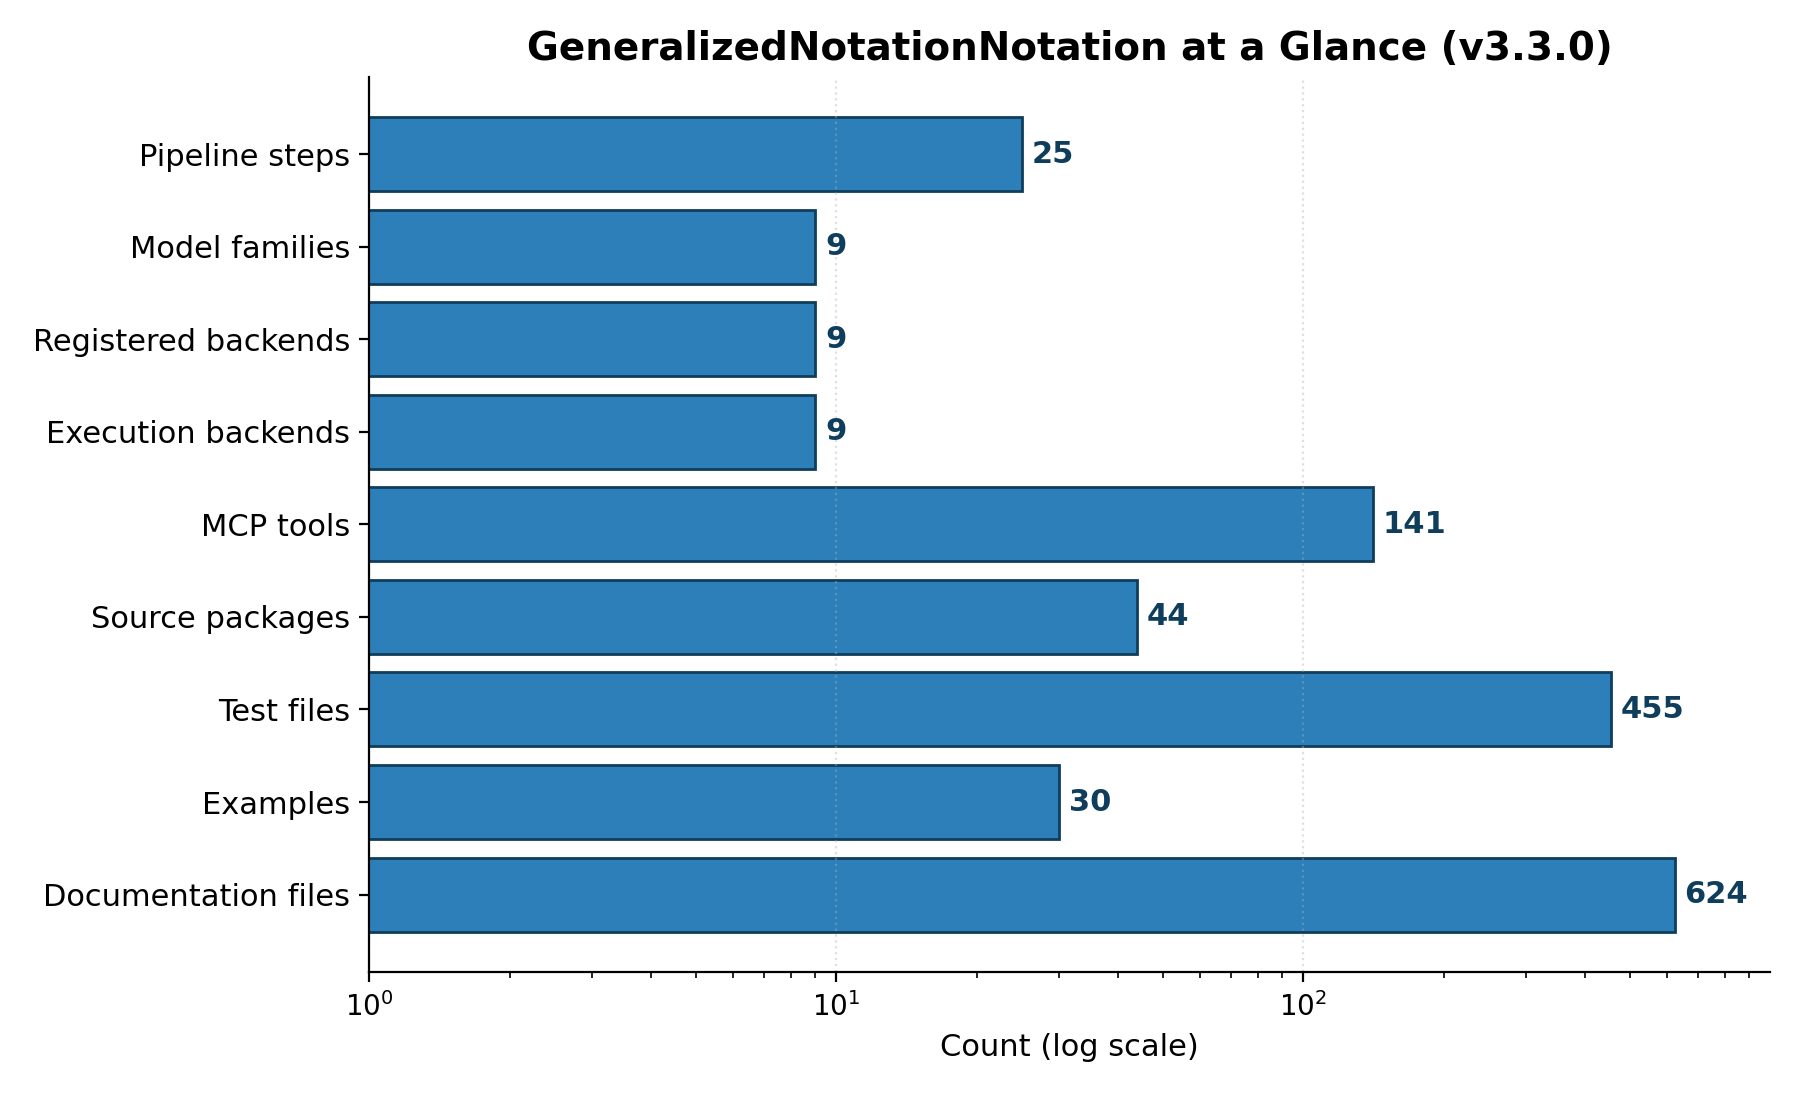
\includegraphics[width=0.8\linewidth,height=0.5\textheight,keepaspectratio,alt={Repository-scale counts on a logarithmic axis: pipeline steps, model families, registered backends, execution backends, Model Context Protocol tools, source packages, test files, example models, and documentation files. Every bar is annotated with its exact value, and every value is a producer token read from output/data/manuscript\_variables.json at commit 13bd0637c --- the same token map that substitutes the prose counts, so the figure cannot disagree with the text without failing the figure-freshness suite. The two backend bars are deliberately distinct: registered backends (9) counts render targets, execution backends (9) counts the subset that runs at Step 12. Read the chart as the scale of the surface the pipeline maintains, not as a quality measure.}]{../figures/gnn_repo_metrics.png}
\caption{Repository-scale counts on a logarithmic axis: pipeline steps,
model families, registered backends, execution backends, Model Context
Protocol tools, source packages, test files, example models, and
documentation files. Every bar is annotated with its exact value, and
every value is a producer token read from
\protect\breaktt{output/data/manuscript\_variables.json} at commit
13bd0637c --- the same token map that substitutes the prose counts, so
the figure cannot disagree with the text without failing the
figure-freshness suite. The two backend bars are deliberately distinct:
\emph{registered backends} (9) counts render targets, \emph{execution
backends} (9) counts the subset that runs at Step 12. Read the chart as
the scale of the surface the pipeline maintains, not as a quality
measure.}\label{fig:repo_metrics}
\end{figure}

The test suite comprises 456 test files containing 4896 test functions,
exercising a source base of 680 Python files across 44 packages (197994
lines of source). The pipeline's step modules --- the thin orchestrators
named in tbl.~\ref{tbl:pipeline_steps} --- number 25, one per numbered
step. The Model Context Protocol surface --- which exposes GNN's
capabilities to external agents and tools --- provides 142 tools across
32 modules. The pipeline itself runs as 25 steps (0--24), and 7 figure
artifacts from the rendering of figures, models, and reports are
committed under \texttt{output/}, of which 7 are the manuscript's own.

\subsection{Claim Discipline}\label{claim-discipline}

A claim is manuscript-ready only when it is bound to a verifiable
artifact. Concretely, every claim in this manuscript must rest on one of
four support types:

\begin{itemize}
\tightlist
\item
  A passing test or validator command --- for example the
  semantic-fidelity and cross-framework gates above, which can be re-run
  on demand.
\item
  A generated output produced by a deterministic producer, such as the
  figures rendered from the family and repository scans, or the token
  values emitted by the manuscript-variable producer that backs every
  number on this page.
\item
  A source ledger, manifest, or configuration file that fixes the value
  being claimed.
\item
  A resolved entry in \texttt{references.bib} for any
  external-literature claim \citep{friston2010, parr2022}.
\end{itemize}

The pipeline records its own evidence trail under \texttt{output/}. The
run-level summary is written to \breaktt{output/PIPELINE\_REPORT.md}, and
the per-step execution record --- including which steps ran, their
status, and their artifacts --- is captured in
\breaktt{output/00\_pipeline\_summary}. These are the artifacts a reader
should consult to confirm that the numbers substituted into this section
correspond to a real, reproducible pipeline run rather than to asserted
prose. When a value would otherwise need a literal number with no
producer behind it, the discipline is to omit the number rather than to
hard-code it.

\newpage

\section{Reproducibility}\label{sec:reproducibility}

Reproducibility in GNN is not an aspiration layered on top of the
system; it is the operating contract that the pipeline enforces. The
0--24 processing steps are deterministic given a model specification and
a target directory, and every published claim in this manuscript is
traceable to a command that regenerates the underlying artifact. This
section lists only commands that exist in the repository, so that a
reader with a clean checkout can reproduce the pipeline, the validation
gates, and this manuscript itself.

\subsection{Pipeline Smoke Run}\label{pipeline-smoke-run}

The fastest way to confirm a working installation is to drive the full
pipeline over the discrete model family without invoking the optional
LLM steps:

\begin{Shaded}
\begin{Highlighting}[]
\ExtensionTok{uv}\NormalTok{ run python src/gnn/main.py }\AttributeTok{{-}{-}target{-}dir}\NormalTok{ input/gnn\_files/discrete }\AttributeTok{{-}{-}output{-}dir}\NormalTok{ /tmp/gnn{-}smoke }\AttributeTok{{-}{-}skip{-}llm}
\end{Highlighting}
\end{Shaded}

This parses the discrete GNN files, runs visualization and rendering
across the maintained backends, and writes all artifacts under the
chosen output directory. The \texttt{-\/-skip-llm} flag keeps the run
hermetic and free of external API calls: the non-LLM steps all execute,
the steps that would read the skipped LLM outputs record that as a
warning, and the run exits 2 --- the pipeline's documented warning code
(0 success, 1 error, 2 warning) --- rather than 0. To exercise every
registered family rather than a single one, drive the manifest through
the model-family acceptance gate given below: pointing
\texttt{-\/-target-dir} at \texttt{input/gnn\_files} covers that tree's
11 corpus directories. All 9 registered family target directories lie
inside that tree, so a single invocation reaches every registered
family.

The discrete family exercises the categorical kind end to end. The
continuous linear-Gaussian kind smoke-runs the same way, and the
contrast between the two runs is itself a check of the per-kind
contract:

\begin{Shaded}
\begin{Highlighting}[]
\ExtensionTok{uv}\NormalTok{ run python src/gnn/main.py }\AttributeTok{{-}{-}target{-}dir}\NormalTok{ input/gnn\_files/continuous }\AttributeTok{{-}{-}output{-}dir}\NormalTok{ /tmp/gnn{-}smoke{-}continuous }\AttributeTok{{-}{-}skip{-}llm}
\end{Highlighting}
\end{Shaded}

This parses the continuous specifications, and the render and execute
steps fan them out to the continuous-capable backends --- where they
render as linear-Gaussian models and run as filtering (and, for the
closed-loop exemplar, belief-steering) programs --- while the
categorical-only backends record explicit \texttt{unsupported} statuses
rather than failures. A reader comparing the two receipts sees the kind
taxonomy behaving as described in sec.~\ref{sec:system_context}: same
pipeline, same steps, per-kind rendering and execution reach.

\subsection{Validation Gates}\label{validation-gates}

GNN's reproducibility guarantees rest on a small set of strict,
deterministic gates that bind the manuscript's quantitative claims to
recomputable ledgers. The model-family acceptance gate runs the
maintained families declared in the manifest and fails on any
regression:

\begin{Shaded}
\begin{Highlighting}[]
\ExtensionTok{uv}\NormalTok{ run python scripts/run\_model\_family\_acceptance.py }\DataTypeTok{\textbackslash{}}
  \AttributeTok{{-}{-}manifest}\NormalTok{ input/model\_family\_manifest.json }\DataTypeTok{\textbackslash{}}
  \AttributeTok{{-}{-}output{-}dir}\NormalTok{ output/model\_family\_acceptance }\AttributeTok{{-}{-}strict}
\end{Highlighting}
\end{Shaded}

The semantic-fidelity gate verifies that a parse \texorpdfstring{\ensuremath{\to}}{->} serialize \texorpdfstring{\ensuremath{\to}}{->} parse
round trip preserves variables, edges, dimensions, parameter shapes,
equations, time semantics, and ontology mappings across the 9 model
families; the cross-framework gate profiles the 7 maintained backends
(PyMDP, RxInfer.jl, JAX, NumPyro, PyTorch, ActiveInference.jl, DisCoPy)
--- refusing any framework outside that set --- and records explicit
compatible and unsupported statuses rather than silently degrading. Both
write their ledgers to an output directory of your choosing:

\begin{Shaded}
\begin{Highlighting}[]
\ExtensionTok{uv}\NormalTok{ run python scripts/run\_semantic\_fidelity\_gate.py }\DataTypeTok{\textbackslash{}}
  \AttributeTok{{-}{-}manifest}\NormalTok{ input/model\_family\_manifest.json }\DataTypeTok{\textbackslash{}}
  \AttributeTok{{-}{-}output{-}dir}\NormalTok{ output/semantic\_fidelity }\AttributeTok{{-}{-}strict}
\ExtensionTok{uv}\NormalTok{ run python scripts/run\_cross\_framework\_reliability.py }\DataTypeTok{\textbackslash{}}
  \AttributeTok{{-}{-}manifest}\NormalTok{ input/model\_family\_manifest.json }\DataTypeTok{\textbackslash{}}
  \AttributeTok{{-}{-}output{-}dir}\NormalTok{ output/cross\_framework }\AttributeTok{{-}{-}strict}
\end{Highlighting}
\end{Shaded}

Under \texttt{-\/-strict}, each gate exits non-zero on the first
mismatch, so these commands double as assertions in an automated
reproduction run. Code-quality reproducibility is enforced separately
through the developer command reference: \texttt{just\ lint} runs the
Ruff linter over \texttt{src} and \texttt{scripts}, and the broader
\texttt{just\ quality} recipe chains formatting, terminology,
documentation, type, and security checks for a full pre-commit gate.

\subsection{Manuscript
Reproducibility}\label{manuscript-reproducibility}

This manuscript is itself a reproducible artifact. Every quantitative
value in the prose --- the pipeline step count, the family and backend
counts, the source and test inventories --- is a token rather than a
hard-coded literal, and the deterministic producer regenerates all of
them from the tracked files at the current commit:

\begin{Shaded}
\begin{Highlighting}[]
\ExtensionTok{uv}\NormalTok{ run python scripts/z\_generate\_manuscript\_variables.py}
\end{Highlighting}
\end{Shaded}

That command recomputes the \{\{\ldots\}\} tokens, persists them to
\breaktt{output/data/manuscript\_variables.json} for audit, and hydrates
the manuscript sources into \breaktt{output/manuscript/}. The
manuscript's own figures are rebuilt from the same token map:

\begin{Shaded}
\begin{Highlighting}[]
\ExtensionTok{uv}\NormalTok{ run python }\AttributeTok{{-}m}\NormalTok{ scripts.manuscript\_build\_figures}
\end{Highlighting}
\end{Shaded}

The hydrated sources are then rendered to PDF by the docxology
template's render stage. That stage lives in a separate checkout, with
this repository symlinked into it at
\breaktt{projects/active/GeneralizedNotationNotation}; run from the
template root:

\begin{Shaded}
\begin{Highlighting}[]
\ExtensionTok{uv}\NormalTok{ run }\AttributeTok{{-}{-}frozen}\NormalTok{ python scripts/pipeline/stage\_03\_render.py }\DataTypeTok{\textbackslash{}}
  \AttributeTok{{-}{-}project}\NormalTok{ GeneralizedNotationNotation}
\end{Highlighting}
\end{Shaded}

The render needs a LaTeX installation providing the packages listed in
\breaktt{manuscript/preamble.md} plus \texttt{seqsplit}; the template
guards \texttt{seqsplit} with \texttt{\textbackslash{}IfFileExists}, so
a missing copy degrades rather than failing the build.

Because the variables file is regenerated before rendering, the counts
in the rendered PDF track the repository state at the commit recorded in
\breaktt{output/data/manuscript\_variables.json} (13bd0637c): a code
change that alters, for example, the test inventory (456 test files,
4896 test functions) propagates into the prose on the next regeneration
without any manual editing.

\subsection{Reproducibility Contract}\label{reproducibility-contract}

\begin{itemize}
\tightlist
\item
  Do not cite results that cannot be regenerated or directly traced to a
  command in this repository.
\item
  Keep generated outputs under \texttt{output/} and maintained
  manuscript source under \texttt{manuscript/}; treat everything in
  \texttt{output/} as disposable and regeneratable.
\item
  Express every quantitative claim in the prose as a double-brace
  \texttt{\{\{...\}\}} token substituted by
  \breaktt{scripts/z\_generate\_manuscript\_variables.py}, never as a
  hard-coded number.
\item
  Keep private data, credentials, and unpublished sensitive details out
  of the manuscript and out of version control.
\item
  Record the exact verification commands --- the smoke run, the
  acceptance and fidelity gates, and \texttt{just\ lint} --- before
  marking this manuscript publication-ready.
\end{itemize}

\newpage

\section{Limitations and Next Steps}\label{sec:limitations_next_steps}

\subsection{Current Limitations}\label{current-limitations}

GNN 3.3.0 is a working system with deliberately scoped boundaries, and
it is worth stating those boundaries plainly rather than implying
broader completeness than the artifacts support. The reliability gates
that underpin our confidence in the system --- the semantic-fidelity
ledger and the cross-framework reliability ledger --- are reproducible
by command and recorded against the 9 model families, but this
manuscript does not assert a particular full-suite pass rate as a
headline number. Pass and skip counts shift with the local toolchain,
the presence or absence of optional simulation dependencies, and whether
the optional Ollama integration paths are exercised, so we treat the
reproducing command as the durable claim and leave the run-specific
tallies to the ledgers and execution traces that the pipeline writes
alongside each run. A reader who wants a number should regenerate it in
their own environment rather than trust a transcribed digit here.

A second limitation lives at the boundary between the model families and
the rendering backends. GNN registers 9 simulation backends, but
coverage across the family-by-backend matrix is intentionally uneven,
and the gaps are recorded as explicit \emph{profiled-unsupported}
statuses rather than silently omitted. The cross-framework acceptance
check is anchored on the continuous family, where JAX, NumPyro,
RxInfer.jl are compared directly; the continuous and hierarchical
families, by contrast, carry profiled-unsupported markers at the render
and execute steps (Steps 11 and 12) for backends that cannot yet
faithfully realize their continuous-state or temporal-depth structure.
This is honest bookkeeping, not a defect to be hidden: an unsupported
status with a recorded reason is more trustworthy than a forced
translation that quietly misrepresents the model. It also reflects the
state of the surrounding literature, where expected-free-energy
formulations, variational-inference reductions, and hierarchical
active-inference methods are still being actively refined rather than
collapsed into one settled executable recipe
\citep{champion2024reframingEfe, nuijten2026typeInference, rangarajan2026hierarchicalSuccessor}.
The practical consequence is that not every model expressible in the GNN
syntax can be executed on every registered backend today, and authors
should consult the profiled-unsupported ledger that
\breaktt{scripts/run\_model\_family\_acceptance.py} writes --- the
command is given in sec.~\ref{sec:reproducibility} --- before assuming a
given family will round-trip through a given framework. The per-kind
shape of that matrix matters as much as its gaps: the categorical-only
backends report the continuous linear-Gaussian kind \texttt{unsupported}
by declared capability rather than by accident, the structural kind is
render-only by design on every backend, and the recursive corpus is
reserved for bounded autonomous runs and holds no committed models yet
--- boundaries recorded where the kinds are defined
(sec.~\ref{sec:model_kinds}) rather than discovered mid-run.

A third limitation is one of scope rather than capability. The formal
account in sec.~\ref{sec:system_context} fixes each kind's
parameterization as given --- the categorical tensors \texttt{A},
\texttt{B}, \texttt{C}, \texttt{D}, and \texttt{E} of the discrete kind
and the system matrices, Gaussian prior, and optional control
declarations of the linear-Gaussian kind --- and states only
belief-level inference: state and policy inference for the categorical
kind (eq.~\ref{eq:vfe}, eq.~\ref{eq:efe}) and fixed-parameter filtering
and control for the continuous kind. GNN can also express
\emph{parameter} learning: a matrix may be declared as a latent variable
with a Dirichlet prior, and the repository ships both a corpus model
that does so
(\breaktt{input/gnn\_files/learning/dirichlet\_likelihood\_learning.md},
which learns its likelihood matrix \texttt{A} from observations by joint
variational message passing) and the renderer strategy that emits code
for it (\breaktt{src/gnn/render/rxinfer/\_strategies\_learning.py}). That
corpus directory is registered in no manifest family --- the
unregistered set is exactly \breaktt{input/gnn\_files/learning},
\breaktt{input/gnn\_files/recursive} --- so parameter learning is
exercised by neither the semantic-fidelity nor the cross-framework
ledger and carries no figure or table in this manuscript. We state it
here as implemented-but-out-of-scope rather than leave the omission to
be inferred from the family tables.

Finally, several capabilities depend on optional dependencies that are
not part of the minimal install. The simulation frameworks themselves,
the audio sonification path, the LLM-enhanced analysis step, and the
interactive visualization step all require extra packages that a lean
checkout will not have, and the corresponding pipeline steps degrade to
recorded skips rather than failures when those dependencies are absent.
This keeps the core parse-validate-export-visualize spine runnable in
constrained environments, but it means a full 0--24 traversal of all 25
steps reflects the optional surface that a particular machine has
installed. We consider this an acceptable engineering trade for
portability, but it is a limitation a reader should hold in mind when
interpreting any single end-to-end run.

\subsection{Next Steps}\label{next-steps}

The roadmap is concrete and staged. The current release is GNN 3.3.0
(``One Corpus'', 2026-09-06). It builds on the three safe-by-design
orchestration contracts introduced in GNN 3.0.0, which generate and
validate data only, with no live infrastructure mutation. The first is
\emph{durable observation streams}: file- and array-backed stream
manifests (content-checksummed) with replayable execution traces, so
that an extended run can be observed, paused, and re-derived
deterministically before any live sensor or device-backed stream is ever
introduced. The second is \emph{resumable run sessions}: run-session
manifests with atomic checkpoint/resume, status inspection, and
cancellation-safe cleanup so that extended model-family acceptance runs
can be interrupted and resumed without corrupting partial state. The
third is \emph{auditable container plans}: generating hardened container
plans with an explicit static security-review and rollback descriptor,
deliberately stopping short of mutating any real cluster. Each contract
is covered by tests over real objects with negative controls and a
strict acceptance gate, additive live wiring connects them to the
session-acceptance and run-manifest paths, and three new Model Context
Protocol tools expose them. The unifying discipline across all three is
that orchestration becomes more capable only as fast as it becomes more
inspectable.

The next major release pushes toward bounded autonomy, and it is gated
behind the 3.0.0 orchestration work for good reason. The intent is to
promote today's proposal-only candidate-scoring machinery --- which
already ranks candidate patches using the existing validators,
model-family ledgers, and interpretability reports --- toward
\emph{reviewed self-editing of GNN files}. Crucially, the design keeps a
human in the loop: edits are proposed and applied only after explicit
user approval, with no automatic source mutation, and the autonomy is
wrapped in policy, rollback, and audit controls before any
self-modifying or distributed action is permitted. This continues the
same principle that governs the rest of the system, in the lineage of
active-inference accounts of self-organizing systems that act to
minimize free energy under explicit generative models
\citep{friston2010, parr2022}: an agent should expand its license to act
only in proportion to the reviewability of what it does. The
next-release items are not claimed as complete here; they are the
recorded direction of travel, and each will be evidenced by its own
gates when it lands, just as the 3.0.0 contracts are evidenced by theirs
today. On the model-kind axis the same staging applies: extending native
hierarchical rendering beyond the two-level strategies, broadening
continuous reach across the remaining registered backends, and
populating the reserved recursive corpus each arrive with their own gate
evidence rather than by prose assertion.

\newpage

\section{Supplemental Source Surface}\label{sec:source_surface}

This supplement records the top-level source surfaces a reader or
reviewer should inspect before turning any prose in the main manuscript
into a verifiable claim. Each surface below is authored material under
version control; the generated artifacts it produces are described
separately so that the boundary between hand-written source and
reproducible output stays explicit.

The \texttt{src/} tree is the executable core of GNN. It is organized
into 44 Python packages spanning 680 source files and roughly 197994
lines of code. Alongside these packages sit the 25 top-level step
modules (0--24) that implement the numbered pipeline as thin
orchestrators delegating into the packages, each module owning one stage
of the progression from a parsed GNN text model through visualization,
type checking, code export, and executable cognitive simulation. Every
claim the manuscript makes about pipeline behavior should be traceable
to one of these step modules rather than to descriptive prose alone.

The \texttt{input/} tree holds the model corpora that exercise the
pipeline. Its \texttt{gnn\_files/} subtree contains 11 corpus
directories organized by model family, together totaling 30 example
files --- 27 discrete-state specifications and 3 continuous
linear-Gaussian specifications, the partition the manuscript's
model-kind accounting uses (sec.~\ref{sec:model_kinds}). The cold-start
index \breaktt{input/gnn\_files/INDEX.md} catalogues every exemplar with
its kind and task folder, and the \texttt{recursive/} directory is
reserved for bounded \texttt{-\/-autonomous} proposal-loop runs, holding
no committed models. Every model file under \texttt{input/} lives in
that subtree, so the 30-file count covers the whole tree. A
\breaktt{model\_family\_manifest.json} enumerates the 9 registered
families and their target directories. This manifest is the
authoritative registry that downstream steps and the manuscript variable
producer read when they report family counts and cross-framework
coverage; it should be consulted directly rather than inferred from
directory listings.

The \texttt{scripts/} tree contains the thin orchestrators that gate and
reproduce the project. These include the acceptance scripts that confirm
the pipeline runs end to end, the reliability gates that enforce
determinism and coverage expectations, and the manuscript variable
producer (\breaktt{src/gnn/manuscript/variables.py} driven from this
layer) that emits the double-brace \texttt{\{\{...\}\}} token values
consumed throughout the manuscript. Treating these scripts as the source
of reproduction commands keeps reported numbers bound to what the code
actually computes.

The \texttt{docs/} tree is the prose and reference surface, comprising
624 files of specification, tutorial, and design documentation for the
GNN language and its Active Inference grounding \citep{gnn2023}. It is
the place to verify that a manuscript statement about GNN syntax or
semantics matches the documented language rather than a convenient
paraphrase.

The \texttt{output/} tree collects per-step pipeline artifacts: the data
dumps, intermediate representations, validation reports, and the 7
figure artifacts committed under it. Everything here is disposable and
reproducible from the surfaces above, so it should be read as evidence
of a run rather than as authored source. Notably,
\breaktt{output/data/manuscript\_variables.json} is where the
manuscript's substituted token values are materialized.

\subsection{Authored Source Versus Generated
Output}\label{authored-source-versus-generated-output}

\texttt{src/}, \texttt{scripts/}, \texttt{input/}, \texttt{docs/} and
\texttt{manuscript/} are authored and reviewed; everything under
\texttt{output/} is generated and disposable, including
\breaktt{output/manuscript/}, which holds the token-substituted copies of
the \texttt{manuscript/} sources rather than the sources themselves. The
commands that regenerate the output surfaces are listed in
sec.~\ref{sec:reproducibility}: the smoke run for the per-step
artifacts, \breaktt{scripts/z\_generate\_manuscript\_variables.py} for
the token map and the hydrated sections,
\breaktt{scripts.manuscript\_build\_figures} for the 7 manuscript
figures, and the template render stage for the PDF. Which values become
tokens is not a matter of taste: any quantity the producer can derive
from a source surface is a token,
\breaktt{scripts/check\_manuscript\_tokens.py} fails the build when a
section hard-codes one instead, and the resulting 93-entry map is
committed at \breaktt{output/data/manuscript\_variables.json} for audit.
External references are resolved from
\breaktt{manuscript/references.bib}, which the same gate cross-checks
against every citation key in the prose. This manuscript quotes no
private or unpublished material.

\newpage

\section{Symbols and Glossary}\label{sec:symbols_glossary}

This glossary defines the Generalized Notation Notation (GNN) language
constructs used to specify generative models, together with the Active
Inference symbols those constructs carry across the model kinds of
sec.~\ref{sec:model_kinds}. Definitions follow the GNN syntax
specification and the exemplar specifications distributed with the
repository --- the discrete POMDP exemplars and the continuous
linear-Gaussian exemplars alike --- and they align with the standard
formulations of both kinds \citep{gnn2023, dacosta2020, parr2022}.

\subsection{Language Constructs}\label{language-constructs}

A GNN file is an ordered, UTF-8 Markdown document whose level-2 headers
name required and optional sections. The strict schema validator
enforces section order, declaration grammar, and connection syntax; the
constructs below are the load-bearing sections a parser must recognize;
they are catalogued in tbl.~\ref{tbl:gnn_constructs}.

\begin{longtable}[]{@{}
  >{\raggedright\arraybackslash}p{(\linewidth - 2\tabcolsep) * \real{0.5000}}
  >{\raggedright\arraybackslash}p{(\linewidth - 2\tabcolsep) * \real{0.5000}}@{}}
\caption{The GNN language constructs a conforming parser must recognize,
with the meaning each carries. The first rows are the required sections
that pin a model's identity, variables, and factor graph; the optional
sections that follow carry parameterization, ontology bindings, timing,
equations, and provenance. The operator rows are the connection
vocabulary the \protect\texttt{Connections} section is written in ---
directed \protect\texttt{A\textgreater{}B}, undirected
\protect\texttt{A-B}, and their labeled v1.1 forms --- and
\protect\texttt{default=…} supplies initialization hints. Definitions
follow the GNN syntax specification and the exemplar specifications
under \protect\texttt{input/gnn\_files}, and the strict schema validator
enforces section order and declaration grammar before any downstream
step runs. The construct vocabulary is deliberately kind-agnostic: the
same \protect\texttt{StateSpaceBlock}, \protect\texttt{Connections}, and
operator syntax declare a discrete categorical model, a continuous
linear-Gaussian model, or a composed multi-agent or hierarchical one ---
what differs between kinds is which matrix names the block declares, as
tbl.~\ref{tbl:actinf_symbols}
details.}\label{tbl:gnn_constructs}\tabularnewline
\toprule\noalign{}
\begin{minipage}[b]{\linewidth}\raggedright
Construct
\end{minipage} & \begin{minipage}[b]{\linewidth}\raggedright
Meaning
\end{minipage} \\
\midrule\noalign{}
\endfirsthead
\toprule\noalign{}
\begin{minipage}[b]{\linewidth}\raggedright
Construct
\end{minipage} & \begin{minipage}[b]{\linewidth}\raggedright
Meaning
\end{minipage} \\
\midrule\noalign{}
\endhead
\bottomrule\noalign{}
\endlastfoot
\texttt{\#\#\ GNNSection} & Required short identifier for the model
block (no spaces, e.g.~\texttt{ActInfPOMDP}). \\
\breaktt{\#\#\ GNNVersionAndFlags} & Required version declaration
(\texttt{GNN\ v1} or \texttt{GNN\ v1.1}) with optional flags. \\
\texttt{\#\#\ ModelName} & Required human-readable title of the
generative model. \\
\breaktt{\#\#\ StateSpaceBlock} & Required block declaring every variable
and matrix as \texttt{NAME{[}dim,\ …,\ type=…{]}}, one per line --- the
block whose declared vocabulary fixes the model's kind. \\
\texttt{\#\#\ Connections} & Required edge list relating state-space
variables, expressing the model's factor graph. \\
\breaktt{\#\#\ ModelAnnotation} & Optional free-text description of the
model's modalities, factors, and assumptions. \\
\breaktt{\#\#\ InitialParameterization} & Optional concrete numeric
values for declared matrices and vectors. \\
\breaktt{\#\#\ ActInfOntologyAnnotation} & Optional bindings from each
variable to a CamelCase Active Inference ontology term. \\
\breaktt{\#\#\ ModelParameters} & Optional key-value dimensions
(e.g.~\breaktt{num\_hidden\_states}, \texttt{num\_obs},
\texttt{num\_actions}) consumed by code generators. \\
\texttt{\#\#\ Time} & Optional dynamics declaration: a time variable
plus \texttt{Dynamic}/\texttt{Static},
\texttt{Discrete}/\texttt{Continuous}, and \breaktt{ModelTimeHorizon}. \\
\texttt{\#\#\ Equations} & Optional LaTeX-rendered formulas defining
model dynamics and the relationships between declared variables;
round-tripped by the semantic-fidelity gate. \\
\texttt{\#\#\ Footer} & Optional closing section that terminates the
file and lets a reader or parser enter it from either end. \\
\texttt{\#\#\ Signature} & Optional provenance block carrying a
cryptographic signature over the specification. \\
\texttt{NAME{[}d\texorpdfstring{\textsubscript{1}}{1},d\texorpdfstring{\textsubscript{2}}{2},…,type=…{]}} & A variable or tensor declaration;
dimensions are positive integers or named references, and a
\texttt{type} (\texttt{float}, \texttt{int}, \texttt{bool}) is
required. \\
\texttt{A\textgreater{}B} & Directed (causal) connection operator: edge
from \texttt{A} to \texttt{B}, e.g.~\texttt{D\textgreater{}s} (a prior
conditions a hidden state) or \texttt{F\textgreater{}x} (a transition
matrix drives a continuous state). \\
\texttt{A-B} & Undirected (bidirectional) connection operator,
e.g.~\texttt{s-A} (a hidden state participates in the likelihood
mapping). \\
\texttt{A\textgreater{}B:label} / \texttt{A-B:label} & A v1.1 annotated
edge; the trailing label documents the relation and is preserved but may
be ignored for structural validation. \\
\texttt{default=…} & A v1.1 declaration hint (\texttt{uniform},
\texttt{zeros}, \texttt{ones}, \texttt{eye}, \texttt{random}) supplying
an initialization for a matrix or vector. \\
\end{longtable}

\subsection{Symbols by Model Kind}\label{symbols-by-model-kind}

The exemplar specifications declare the generative-model components of
Active Inference, mapping each GNN variable to its probabilistic meaning
\citep{dacosta2020, smith2022, parr2022}. Because the notation spans
model kinds, the same letter can name different objects in different
kinds --- most prominently \texttt{F}, which is the variational free
energy of eq.~\ref{eq:vfe} in the discrete kind and the state-transition
matrix of eq.~\ref{eq:lgssm_state} in the continuous kind --- so each
row of tbl.~\ref{tbl:actinf_symbols} names the kind its reading belongs
to and the equation in sec.~\ref{sec:system_context} that fixes it, and
the glossary and the formal statement cannot drift apart.

\begin{longtable}[]{@{}
  >{\raggedright\arraybackslash}p{(\linewidth - 2\tabcolsep) * \real{0.5000}}
  >{\raggedright\arraybackslash}p{(\linewidth - 2\tabcolsep) * \real{0.5000}}@{}}
\caption{The Active Inference symbols a GNN specification carries,
scoped by model kind and bound to the equation of
sec.~\ref{sec:system_context} that fixes each role. Read the
discrete-kind rows as the categorical generative-model tensors
(likelihood, controlled transitions, log-preferences, prior over initial
states, habit prior) with \protect\texttt{s}, \protect\texttt{o},
\protect\texttt{\texorpdfstring{\ensuremath{\pi}}{pi}}, and \protect\texttt{u} as the inference variables
and \protect\texttt{F} and \protect\texttt{G} as the two free-energy
functionals minimized at eq.~\ref{eq:vfe} and eq.~\ref{eq:efe}; read the
continuous-kind rows as the linear-Gaussian parameterization --- system
matrices, covariances, Gaussian prior, and the optional closed-loop
declarations of eq.~\ref{eq:closed_loop}. The rows where one letter
carries two kind-scoped readings (\protect\texttt{F},
\protect\texttt{u}, \protect\texttt{t}) are deliberate: the notation
reuses a compact alphabet across kinds, and the declared matrix
vocabulary of the \protect\texttt{StateSpaceBlock} --- not the letter
alone --- is what fixes the reading, which is exactly what the kind
classification of sec.~\ref{sec:model_kinds} computes. Use the table as
a decoding key when reading a \protect\texttt{StateSpaceBlock}: every
declared matrix name should map to exactly one kind-scoped row here, and
the \protect\breaktt{\#\#\ ActInfOntologyAnnotation} bindings described
below are what make that mapping machine-checkable
downstream.}\label{tbl:actinf_symbols}\tabularnewline
\toprule\noalign{}
\begin{minipage}[b]{\linewidth}\raggedright
Symbol
\end{minipage} & \begin{minipage}[b]{\linewidth}\raggedright
Meaning
\end{minipage} \\
\midrule\noalign{}
\endfirsthead
\toprule\noalign{}
\begin{minipage}[b]{\linewidth}\raggedright
Symbol
\end{minipage} & \begin{minipage}[b]{\linewidth}\raggedright
Meaning
\end{minipage} \\
\midrule\noalign{}
\endhead
\bottomrule\noalign{}
\endlastfoot
\texttt{A} & Discrete kind: likelihood (observation) matrix encoding
\(P(o \mid s)\), a column-stochastic map from hidden states to
observation outcomes (eq.~\ref{eq:likelihood}). \\
\texttt{B} & Discrete kind: transition tensor encoding
\(P(s' \mid s, u)\), one column-stochastic slice per action in the
canonical \texttt{B{[}next\_state{]}{[}previous\_state{]}{[}action{]}}
order (eq.~\ref{eq:transition}). \\
\texttt{C} & Discrete kind: preference vector --- log-preferences over
observation outcomes that bias the agent toward preferred outcomes
(eq.~\ref{eq:preference}). \\
\texttt{D} & Discrete kind: prior vector over initial hidden states
(eq.~\ref{eq:prior}). \\
\texttt{E} & Discrete kind: habit vector --- an initial policy prior
over actions, entering the policy posterior (eq.~\ref{eq:policy}). \\
\texttt{s} & Discrete kind: current hidden-state distribution;
\texttt{s\_prime} (\texttt{s\textquotesingle{}}) is the next
hidden-state distribution. \\
\texttt{o} & Discrete kind: current observation, an integer index over
outcome modalities. \\
\texttt{\texorpdfstring{\ensuremath{\pi}}{pi}} & Discrete kind: policy --- a distribution over actions
inferred from expected free energy (eq.~\ref{eq:policy}). \\
\texttt{u} & Discrete kind: the selected (sampled) action, sampled from
the policy posterior. Continuous kind: the control input added to the
state each step (eq.~\ref{eq:lgssm_state}). \\
\texttt{F} & Discrete kind: variational free energy, minimized during
state inference (eq.~\ref{eq:vfe}) \citep{friston2010}. Continuous kind:
the state-transition matrix of the linear-Gaussian model
(eq.~\ref{eq:lgssm_state}). \\
\texttt{G} & Discrete kind: expected free energy per policy, minimized
during policy inference to score candidate actions (eq.~\ref{eq:efe})
\citep{dacosta2020}. \\
\texttt{t} & Discrete time step; the horizon \(T\) bounds the product in
eq.~\ref{eq:generative_model}. Continuous kind: the time index of the
state-space model. \\
\texttt{H} & Continuous kind: observation matrix mapping the latent
state to the observation (eq.~\ref{eq:lgssm_obs}). \\
\texttt{Q} & Continuous kind: process-noise covariance of the state
evolution (eq.~\ref{eq:lgssm_state}). \\
\texttt{R} & Continuous kind: observation-noise covariance of the
readout (eq.~\ref{eq:lgssm_obs}). \\
\texttt{x} & Continuous kind: the Gaussian latent state \(x_t\);
\texttt{x{[}2,1,type=float{]}} in the navigation exemplar declares a
two-dimensional position. \\
\texttt{y} & Continuous kind: the continuous observation read out
linearly from the state (eq.~\ref{eq:lgssm_obs}). \\
\texttt{prior\_mean} & Continuous kind: prior mean \(\mu_0\) over the
initial latent state (eq.~\ref{eq:lgssm_state}). \\
\texttt{prior\_cov} & Continuous kind: prior covariance \(\Sigma_0\)
over the initial latent state (eq.~\ref{eq:lgssm_state}). \\
\texttt{goal\_mean} & Continuous kind: preferred state \(\mu^\star\) the
closed-loop controller steers toward (eq.~\ref{eq:closed_loop}). \\
\texttt{control\_gain} & Continuous kind: scalar proportional gain \(k\)
on the belief error in the closed loop (eq.~\ref{eq:closed_loop}). \\
\end{longtable}

\subsection{Ontology Bindings and
Implementations}\label{ontology-bindings-and-implementations}

The \breaktt{\#\#\ ActInfOntologyAnnotation} section binds each variable
to a canonical term --- \breaktt{A=LikelihoodMatrix},
\breaktt{B=TransitionMatrix}, \breaktt{C=LogPreferenceVector},
\breaktt{D=PriorOverHiddenStates}, \texttt{s=HiddenState},
\texttt{o=Observation}, \texttt{\texorpdfstring{\ensuremath{\pi}}{pi}=PolicyVector} in the discrete
exemplars; \breaktt{F=StateTransitionMatrix},
\breaktt{H=ObservationMatrix}, \breaktt{Q=ProcessNoiseCovariance},
\breaktt{R=ObservationNoiseCovariance}, \breaktt{prior\_mean=PriorMean},
\breaktt{prior\_cov=PriorCovariance}, \breaktt{goal\_mean=PreferredState},
\breaktt{control\_gain=ControlGain}, \breaktt{x=ContinuousHiddenState},
\breaktt{y=ContinuousObservation}, \texttt{u=ControlInput} in the
continuous exemplars --- which downstream pipeline steps use for
semantic analysis and validation. The bindings are per-kind by
construction: a continuous exemplar binds \texttt{F} to
\breaktt{StateTransitionMatrix}, never to a free-energy term, so the
ontology layer carries the same kind-scoped reading
tbl.~\ref{tbl:actinf_symbols} fixes by hand. The same GNN specification
feeds the project's rendering backends --- including the 9 registered
targets (PyMDP, RxInfer.jl, ActiveInference.jl, JAX, DisCoPy, PyTorch,
NumPyro, Stan, bnlearn), of which the 9 listed as executable (PyMDP,
RxInfer.jl, ActiveInference.jl, JAX, DisCoPy, PyTorch, NumPyro, Stan,
bnlearn) also run at Step 12 --- with per-kind reach recorded as
explicit statuses (tbl.~\ref{tbl:framework_capability}) --- so that a
model written once in this notation can be parsed, visualized, and
executed across the 25-step pipeline (0--24) without restating its
mathematics \citep{gnn2023, heins2022, defelice2021}.

\newpage

\section{References}\label{sec:references}

Entries below are resolved by Pandoc from
\href{references.bib}{\breaktt{manuscript/references.bib}} at render
time; \breaktt{scripts/check\_manuscript\_tokens.py} fails the build on a
citation key that file does not define.



\providecommand{\bibsection}{}
\renewcommand{\bibsection}{}

\bibliography{references}
\end{document}
